\documentclass[11pt,a4paper]{article}

\usepackage[utf8]{inputenc}
\usepackage[T1]{fontenc}
\usepackage[english]{babel}
\usepackage{amsmath,amssymb,mathtools,array,booktabs,longtable}
\usepackage{geometry}
\geometry{margin=0.82in}
\usepackage{fancyhdr}
\usepackage{titlesec}
\usepackage{tikz}
\usepackage{pdflscape}
\usetikzlibrary{calc}

\pagestyle{fancy}
\fancyhf{}
\fancyhead[C]{\small Cayley --- Collected Mathematical Papers, Vol.\ VIII}
\fancyfoot[C]{\thepage}
\renewcommand{\headrulewidth}{0.4pt}

\titleformat{\section}{\large\scshape\centering}{}{0em}{}
\titleformat{\subsection}{\normalsize\bfseries\centering}{}{0em}{}
\setlength{\parindent}{1.2em}
\setlength{\parskip}{0.25em}
\allowdisplaybreaks

\newcommand{\sourcepage}[2]{%
  \bigskip
  \noindent\textit{p.~#1 [#2]}%
  \par\smallskip
}
\newcommand{\pagemarker}[2]{\clearpage\noindent\textit{p.~#1 [#2]}\par\medskip}
\newcommand{\papersection}[2]{%
  \section{[#1]}
  \subsection{#2}
}
\newcommand{\fromjournal}[1]{%
  \begin{center}\textit{#1}\end{center}
}
\newcommand{\Det}[1]{\left|\begin{matrix}#1\end{matrix}\right|}
\newcommand{\surf}[1]{\par\smallskip\noindent{\itshape \{Surface $#1$.\}}\par\smallskip}
\newcommand{\qf}[2]{(#1)(#2)^2}
\newcommand{\half}{\tfrac{1}{2}}
\newcommand{\third}{\tfrac{1}{3}}
\newcommand{\quart}{\tfrac{1}{4}}
\newcommand{\eighth}{\tfrac{1}{8}}
\newcommand{\sixteenth}{\tfrac{1}{16}}
\newcommand{\dd}{\,d}
\newcommand{\p}{\mathfrak p}

\begin{document}

% ============================================================
% Printed pages 67--91; source-checked slice expanded on 2026-06-02.
% ============================================================
% Source PDF page 131; printed page 67.
\noindent\textit{p.~67 [498]}

\begin{center}
{\Large 498.}

\vspace{1em}
{\large ON THE INVERSION OF A QUADRIC SURFACE.}

\vspace{1em}
[\textit{From the Quarterly Journal of Pure and Applied Mathematics}, vol. XI. (1871),\\
pp. 283--288.]
\end{center}

The inversion intended to be considered is that by reciprocal radius vectors, viz. if
\(x,y,z\) are rectangular coordinates, and \(r^2=x^2+y^2+z^2\), then \(x,y,z\) are to
be changed into \(\frac{x}{r^2},\frac{y}{r^2},\frac{z}{r^2}\). But it is convenient to
introduce for homogeneity a fourth coordinate \(w,=1\); and the change then is
\(x,y,z\) into
\[
  \frac{xw^2}{r^2},\qquad \frac{yw^2}{r^2},\qquad \frac{zw^2}{r^2}.
\]
Starting from the quadric surface
\[
  \qf{a,b,c,d,f,g,h,l,m,n}{x,y,z,w}=0,
\]
or, what is the same thing,
\[
\begin{aligned}
  &\qf{a,b,c,f,g,h}{x,y,z}
  +2w(lx+my+nz)+dw^2=0,
\end{aligned}
\]
the equation of the inverse surface is
\[
  w^2\qf{a,b,c,f,g,h}{x,y,z}
  +2w(lx+my+nz)r^2+dr^4=0,
\]
where \(r^2=x^2+y^2+z^2\). The inverse surface is thus a quartic having the nodal
conic \(w=0,\ x^2+y^2+z^2=0\) (circle at infinity); and having the node
\(x=0,\ y=0,\ z=0\) (the centre of inversion); or say it is a nodal bicircular
quartic surface, or nodal anallagmatic.

\pagemarker{68}{498}
For \(x,y,z\) write
\[
  x-\half\frac{l}{d}w,\qquad
  y-\half\frac{m}{d}w,\qquad
  z-\half\frac{n}{d}w,
\]
and put for shortness
\[
\begin{gathered}
  lx+my+nz=u,\qquad l^2+m^2+n^2=a,\\
  al+hm+gn=\mathrm{a},\qquad
  hl+bm+fn=\mathrm{b},\qquad
  gl+fm+cn=\mathrm{c},\\
  \qf{a,b,c,f,g,h}{l,m,n}=A.
\end{gathered}
\]
Then
\[
\begin{array}{rcl}
r^2&\hbox{becomes}& r^2-\dfrac{uw}{d}+\dfrac14\dfrac{a}{d^2}w^2,\\[6pt]
lx+my+nz&\hbox{becomes}& u-\dfrac12\dfrac{a}{d}w,\\[6pt]
\qf{a,\ldots}{x,y,z}&\hbox{becomes}&
\qf{a,\ldots}{x,y,z}-(\mathrm{a}x+\mathrm{b}y+\mathrm{c}z)\dfrac{w}{d}
+\dfrac14 A\dfrac{w^2}{d^2}.
\end{array}
\]
Hence the equation is
\[
\begin{aligned}
d\Bigl\{&r^4-2r^2\frac{uw}{d}
+w^2\Bigl(\half\frac{a}{d^2}r^2+\frac{u^2}{d^2}\Bigr)
-\half\frac{auw^3}{d^3}
+\sixteenth\frac{a^2w^4}{d^4}\Bigr\}\\
&+2\Bigl(wr^2-\frac{uw^2}{d}
+\quart\frac{a}{d^2}w^3\Bigr)
\Bigl(u-\half\frac{a}{d}w\Bigr)\\
&+w^2\Bigl\{\qf{a,\ldots}{x,y,z}-(\mathrm{a}x+\mathrm{b}y+\mathrm{c}z)\frac{w}{d}
+\quart A\frac{w^2}{d^2}\Bigr\}=0;
\end{aligned}
\]
viz. arranging and reducing, this is
\[
\begin{aligned}
dr^4
&+w^2\Bigl\{-\half\frac{a}{d}r^2-\frac{u^2}{d}
+\qf{a,\ldots}{x,y,z}\Bigr\}\\
&+w^3\Bigl\{\frac{au}{d^2}-\frac1d(\mathrm{a}x+\mathrm{b}y+\mathrm{c}z)\Bigr\}\\
&+w^4\Bigl\{-\frac3{16}\frac{a^2}{d^3}+\quart A\frac1{d^2}\Bigr\}=0;
\end{aligned}
\]
and we may without loss of generality assume
\[
 -\frac{mn}{d}+f=0,\quad df-mn=0;\qquad
 -\frac{nl}{d}+g=0,\quad dg-nl=0;\qquad
 -\frac{lm}{d}+h=0,\quad dh-lm=0.
\]

\pagemarker{69}{498}
The equation then is
\[
\begin{aligned}
r^4
&+w^2\Bigl\{-\half\frac{a}{d^2}(x^2+y^2+z^2)
+\Bigl(\frac{a}{d}-\frac{l^2}{d^2}\Bigr)x^2
+\Bigl(\frac{b}{d}-\frac{m^2}{d^2}\Bigr)y^2
+\Bigl(\frac{c}{d}-\frac{n^2}{d^2}\Bigr)z^2\Bigr\}\\
&+w^3\Bigl\{\frac{au}{d^3}
-\frac1{d^2}(\mathrm{a}x+\mathrm{b}y+\mathrm{c}z)\Bigr\}\\
&+w^4\Bigl\{-\frac1{4d^3}(l^2a'+m^2b'+n^2c')
+\frac1{16}\frac{a^2}{d^4}\Bigr\}=0.
\end{aligned}
\]
Write
\[
  ad-l^2=a'd,\qquad bd-m^2=b'd,\qquad cd-n^2=c'd.
\]
We have
\[
  \mathrm{a}=al+hm+gn
  =al+\frac{lm^2}{d}+\frac{ln^2}{d}
  =\frac ld(ad-l^2+a),
\]
that is
\[
  \mathrm{a}=la'+\frac{la}{d},
\]
and similarly
\[
  \mathrm{b}=mb'+\frac{ma}{d},\qquad
  \mathrm{c}=nc'+\frac{na}{d}.
\]
Hence also
\[
  A=l^2a'+m^2b'+n^2c'+\frac{a^2}{d},
\]
and the equation is
\[
\begin{aligned}
r^4
&+w^2\Bigl\{\Bigl(-\half\frac{a}{d^2}+\frac{a'}d\Bigr)x^2
+\Bigl(-\half\frac{a}{d^2}+\frac{b'}d\Bigr)y^2
+\Bigl(-\half\frac{a}{d^2}+\frac{c'}d\Bigr)z^2\Bigr\}\\
&+w^3\Bigl\{-\frac{la'}{d^2}x-\frac{mb'}{d^2}y-\frac{nc'}{d^2}z\Bigr\}\\
&+w^4\Bigl\{-\frac1{4d^3}(l^2a'+m^2b'+n^2c')+\frac1{16}\frac{a^2}{d^4}\Bigr\}=0.
\end{aligned}
\]
This is Kummer's form, say
\[
  r^4=4w^2\{a_1x^2+\beta_1y^2+\gamma_1z^2+\delta_1w^2
  +2w(a_1x+b_1y+c_1z)\}.
\]

\pagemarker{70}{498}
Where
\[
\begin{gathered}
-4a_1=-\half\frac{a}{d^2}+\frac{a'}d,\qquad
-4\beta_1=-\half\frac{a}{d^2}+\frac{b'}d,\qquad
-4\gamma_1=-\half\frac{a}{d^2}+\frac{c'}d,\\
-4\delta_1=-\frac1{4d^3}(l^2a'+m^2b'+n^2c')+\frac1{16}\frac{a^2}{d^4},\\
-8a_1=-\frac{la'}{d^2},\qquad
-8b_1=-\frac{mb'}{d^2},\qquad
-8c_1=-\frac{nc'}{d^2}.
\end{gathered}
\]
Hence Kummer's equation
\[
  \delta_1+\lambda^2
  =\frac{a_1^2}{\lambda+a_1}
  +\frac{b_1^2}{\lambda+\beta_1}
  +\frac{c_1^2}{\lambda+\gamma_1},
\]
or say
\[
  64\delta_1+64\lambda^2
  =\frac{256a_1^2}{4\lambda+4a_1}
  +\frac{256b_1^2}{4\lambda+4\beta_1}
  +\frac{256c_1^2}{4\lambda+4\gamma_1},
\]
becomes
\[
\begin{aligned}
64\lambda^2-\frac4{d^3}(l^2a'+m^2b'+n^2c')-\frac{a^2}{d^4}
&=\frac{4l^2a'^2}{d^4(\half\frac{a}{d^2}-\frac{a'}d+4\lambda)}\\
&\quad+\frac{4m^2b'^2}{d^4(\half\frac{a}{d^2}-\frac{b'}d+4\lambda)}
+\frac{4n^2c'^2}{d^4(\half\frac{a}{d^2}-\frac{c'}d+4\lambda)}.
\end{aligned}
\]
This is satisfied by \(4\lambda=-\half\dfrac{a}{d^2}\). Writing therefore
\[
  4\lambda+\half\frac{a}{d^2}=-\frac{\theta}{d},
\]
that is
\[
  8\lambda=-\frac{2\theta}{d}-\frac{a}{d^2},\qquad
  64\lambda^2=\frac{4\theta^2}{d^2}+\frac{4\theta a}{d^3}+\frac{a^2}{d^4},
\]
the equation is
\[
  \frac{4\theta^2}{d^2}+\frac{4\theta a}{d^3}
  -\frac4{d^3}(l^2a'+m^2b'+n^2c')
  =
  \frac{4l^2a'^2}{d^4(-\theta/d-a'/d)}
  +\frac{4m^2b'^2}{d^4(-\theta/d-b'/d)}
  +\frac{4n^2c'^2}{d^4(-\theta/d-c'/d)}.
\]
Viz. this is
\[
  l^2a'+m^2b'+n^2c'-\theta a-\theta^2d
  =
  \frac{l^2a'^2}{\theta+a'}
  +\frac{m^2b'^2}{\theta+b'}
  +\frac{n^2c'^2}{\theta+c'}.
\]

\pagemarker{71}{498}
which is of course satisfied by \(\theta=0\). Moreover the derived equation
\[
  -a-2\theta d
  =-\frac{l^2a'^2}{(\theta+a')^2}
   -\frac{m^2b'^2}{(\theta+b')^2}
   -\frac{n^2c'^2}{(\theta+c')^2}
\]
is also satisfied by \(\theta=0\), so that this is a double root. The equation in fact is
\[
\begin{aligned}
&\{\theta^2d+\theta a-(l^2a'+m^2b'+n^2c')\}
(\theta+a')(\theta+b')(\theta+c')\\
&\quad+\{l^2a'^2(\theta+b')(\theta+c')
+m^2b'^2(\theta+c')(\theta+a')
+n^2c'^2(\theta+a')(\theta+b')\}=0,
\end{aligned}
\]
or, expanding and dividing by \(\theta^2\), this is
\[
\begin{aligned}
&d(\theta+a')(\theta+b')(\theta+c')\\
&\quad+a\{\theta^2+\theta(a'+b'+c')+b'c'+c'a'+a'b'\}\\
&\quad-(l^2a'+m^2b'+n^2c')(\theta+a'+b'+c')\\
&\quad+l^2a'^2+m^2b'^2+n^2c'^2=0,
\end{aligned}
\]
which gives the remaining three roots.

If \(a'=b'=c'\) the equation is
\[
  (\theta+a'+a)(\theta+a')^2=0.
\]
I recall that we have
\[
\begin{gathered}
a,b,c,d,\quad f=\frac{mn}{d},\quad g=\frac{nl}{d},\quad h=\frac{lm}{d},\quad l,m,n,\\
a'=a-\frac{l^2}{d},\qquad b'=b-\frac{m^2}{d},\qquad c'=c-\frac{n^2}{d},\qquad
a=l^2+m^2+n^2,
\end{gathered}
\]
so that the quadric surface is
\[
  d(a'x^2+b'y^2+c'z^2)+(lx+my+nz+dw)^2=0,
\]
and that, \(a_1,\beta_1,\gamma_1,\delta_1,a_1,b_1,c_1\) denoting as before, the
equation of the inverse surface (referred to a different origin) is
\[
  r^4=4w^2\{a_1x^2+\beta_1y^2+\gamma_1z^2+\delta_1w^2
  +2w(a_1x+b_1y+c_1z)\}.
\]

\pagemarker{72}{499}
\begin{center}
{\Large 499.}

\vspace{1em}
{\large ON THE THEORY OF THE CURVE AND TORSE.}

\vspace{1em}
[\textit{From the Quarterly Journal of Pure and Applied Mathematics}, vol. XI. (1871),\\
pp. 294--317.]
\end{center}

The fundamental relations in the theory of the Curve and Torse were first established
in my ``M\'emoire sur les Courbes \`a double courbure et sur les Surfaces
d\'eveloppables,'' Liouv. t. X. (1845), [30] see also Camb. and Dubl. Math. Jour.,
t. IV. (1850), [83], viz. I showed that the systems
\((m,r,\beta,h,n,\gamma)\) and \((r,n,m,x,\alpha,g)\), (the notation is subsequently
explained), each of them satisfied the Plueckerian relations. An additional set of
equations giving the values of
\((\gamma,t,k,q,\gamma',t',k',q')\) was furnished by Dr Salmon's ``Theory of Reciprocal
Surfaces,'' Trans. R. I. Acad., t. XXIII. (1857), see also the Solid Geometry. The
theory as thus established is complete in itself, but it does not take account of
certain singularities \(v,\omega,H,G\); the singularity \(v\) was first considered in my
paper ``On a special sextic Developable,'' Quart. Math. Jour. t. VII. (1865), [373],
(there called \(b\)), and I afterwards endeavoured to take account of the remaining
singularities \(\omega,H,G\). I was in correspondence on the subject with Prof. Cremona,
and the discovery of the complete forms of several of the formulae is due to him.

There has recently appeared a very valuable memoir by M. Zeuthen, ``Sur les
singularit\'es ordinaires d'une courbe gauche et d'une surface d\'eveloppable,'' Annali
di Matem. t. III. (1869); he excludes, however, from consideration the singularity
\(\omega\), and does not throughout attend to \(H,G\).

I propose in the present memoir to reproduce and develope the whole theory.

\begin{center}\textit{Explanations and Notation.}\end{center}

1. We have a singly infinite series of points, lines, and planes; viz. each line passes
through two consecutive points and lies in two consecutive planes; each plane passes
through three consecutive points and contains two consecutive lines; each point

\pagemarker{73}{499}
is the intersection of three consecutive planes and of two consecutive lines. The
points describe and the lines envelope a curve; the lines describe and the planes
envelope a torse; the entire system of points, lines, and planes is thus the system of
the curve and torse. The curve is the edge of regression or cuspidal curve of the
torse; in regard to the curve the points are points (or ineunts), the lines tangents,
and the planes osculating planes: in regard to the torse the points are points on the
edge of regression, the lines generating lines, and the planes tangent planes.

2. Each line of the system is met by a certain number of non-consecutive lines, and
the locus of the points of intersection (or say the locus of the intersection of two
intersecting non-consecutive lines) is a nodal curve on the torse, or say simply it is
the nodal curve. The plane containing the two intersecting non-consecutive lines
envelopes a torse which is called the nexal torse.

3. There is occasion to consider

\(\quad m\), order of the system; this is the number of points of the system which
lie in a given plane; or it is the order of the curve.

\(\quad r\), rank of the system; this is the number of lines of the system which
meet a given line. It is thus the class of the curve; and the order of the torse.

\(\quad n\), class of the system; this is the number of planes of the system which
pass through a given point. It is thus the class of the torse.

\(\quad \alpha\), number of stationary planes; that is, planes each passing through
four consecutive points of the system.

\(\quad \beta\), number of stationary points, that is, points each of them the
intersection of four consecutive planes of the system.

\(\quad g\), number of lines in two planes (that is, lines each of them the intersection
of two non-consecutive planes of the system) contained in a given plane; or say,
number of apparent double planes of the torse.

\(\quad G\), number of double planes, or tropes, of the torse; viz. considering the
torse as the envelope of a variable plane, if the plane in the course of its motion
comes twice into the same position, we have then a double plane or trope.

\(\quad h\), number of lines through two points (that is, lines each through two
non-consecutive points of the system) passing through a given point; or say, number
of apparent double points of the curve.

\(\quad H\), number of double points, or nodes of the curve; viz. considering the curve
as described by a variable point, if the point in the course of its motion comes twice
into the same position we have then a double point or node of the curve.

\(\quad x\), number of points in two lines (that is, points each of them the intersection
of two non-consecutive lines of the system) contained in a given plane; or what is
the same thing, order of nodal curve.

\(\quad y\), number of planes through two lines (that is, planes each containing two
non-consecutive lines of the system) passing through a given point; or what is the
same thing, class of the nexal torse.

\pagemarker{74}{499}
\(\quad v\), number of stationary lines of the system, that is, lines each containing
three consecutive points of the system.

\(\quad \omega\), number of double lines of the system, that is, lines each containing
two pairs of consecutive points of the system.

\(\quad t\), number of points on three lines (that is, points each of them the common
intersection of three non-consecutive lines of the system): these are also triple points
on the curve.

\(\quad \gamma\), number of points of the system, through each of which passes a
non-consecutive line of the system: these are intersections of the curve with the nodal
curve, stationary points on the latter curve.

\(\quad k\), number of apparent double points of nodal curve.

\(\quad q\), class of nodal curve.

\(\quad t'\), number of planes through three lines (that is, planes each of them through
three non-consecutive lines of the system): these are also triple tangent planes of
the torse.

\(\quad \gamma'\), number of planes of the system each of them passing through a
non-consecutive line of the system: these are common tangent planes of the torse
and nexal torse, stationary planes of the latter torse.

\(\quad k'\), number of apparent double planes of nexal torse.

\(\quad q'\), order of nexal torse.

4. The formulae thus contain in all the 21 quantities
\[
m,r,n,\alpha,\beta,g,G,h,H,x,y,v,\omega,t,\gamma,k,q,t',\gamma',k',q'.
\]
My own Plueckerian equations, or, say, the Pluecker-Cayley equations, establish in
all 6 relations between the first 13 quantities, and thus enable the expression of them
in terms of any seven, say of
\[
  m,r,n,G,H,v,\omega,
\]
and the Salmon-Cremona equations then lead to the expressions in terms of these, of
the remaining eight quantities \(t,\gamma,k,q,t',\gamma',k',q'\).

I also consider
\[
  D_m,\ \hbox{the deficiency of the curve},\qquad
  D_x,\ \hbox{the deficiency of the nodal curve}.
\]
I will first consider the equations themselves, and the mere algebraical transformations
thereof; and afterwards the geometrical theory.

\pagemarker{75}{499}
\begin{center}\textit{The Pluecker-Cayley Equations.}\end{center}

5. These are found (as will be further explained) by considering first the cone,
vertex an arbitrary point, which passes through the curve; and secondly, the section
of the torse by an arbitrary plane. We have in the two figures
\[
\begin{array}{c|c}
\textit{Cone.} & \textit{Section.}\\
\begin{array}{rl}
m,&\text{order,}\\
r,&\text{class,}\\
h+H,&\text{double lines,}\\
\beta,&\text{stationary lines,}\\
y+\omega,&\text{double planes,}\\
n+v,&\text{stationary planes}
\end{array}
&
\begin{array}{rl}
n,&\text{class,}\\
r,&\text{order,}\\
g+G,&\text{double tangents,}\\
\alpha,&\text{stationary tangents,}\\
x+\omega,&\text{double points,}\\
m+v,&\text{stationary points.}
\end{array}
\end{array}
\]
Whence the two sets of quantities respectively are connected by the Plueckerian
formulae, viz. these are
\begingroup\tiny\setlength{\arraycolsep}{1pt}
\[
\begin{array}{rcl@{\qquad}rcl}
r&=&m(m-1)-2(h+H)-3\beta,
&
n&=&r(r-1)-2(x+\omega)-3(m+v),\\
n&=&3m(m-2)-6(h+H)-8\beta,
&
\alpha&=&3r(r-2)-6(x+\omega)-8(m+v),\\
g+G&=&\half m(m-2)(m^2-9)
-(m^2-m-6)\{2(h+H)+3\beta\}\\
&&\quad+2(h+H)(h+H-1)+6(h+H)\beta+\tfrac92\beta(\beta-1),
&
g+G&=&\half r(r-2)(r^2-9)\\
&&&\multicolumn{3}{l}{
{}-(r^2-r-6)\{2(x+\omega)+3(m+v)\}
+2(x+\omega)(x+\omega-1)}\\
&&&\multicolumn{3}{l}{
{}+6(x+\omega)(m+v)+\tfrac92(m+v)(m+v-1),}\\
r&=&r(r-1)-2(y+\omega)-3(n+v),
&
r&=&n(n-1)-2(g+G)-3\alpha,\\
\beta-(n+v)&=&3(r-m),
&
\alpha-(m+v)&=&3(n-r),\\
h+H-(y+\omega)&=&\half(r-m)(r+m-9),
&
g+G-(x+\omega)&=&\half(n-r)(n+r-9),\\
\half(r-1)(r-2)-(y+\omega)-(n+v)
&=&\half(m-1)(m-2)-(h+H)-\beta,
&
\half(r-1)(r-2)-(x+\omega)-(m+v)
&=&\half(n-1)(n-2)-(g+G)-\alpha.
\end{array}
\]
\endgroup

\pagemarker{76}{499}
and combining the two systems
\[
\begin{gathered}
\beta=\alpha+2(m-n),\qquad
y=x+(m-n),\\
h+H=g+G+\half(m-n)(m+n-7),\\
\half(m-1)(m-2)-(h+H)-\beta
=\half(n-1)(n-2)-(g+G)-\alpha,\\
\half(r-1)(r-2)-(x+\omega)-(m+v)
=\half(r-1)(r-2)-(y+\omega)-(n+v).
\end{gathered}
\]
6. Taking as data \(r,m,n,G,H,v,\omega\), we find very easily
\[
\begin{aligned}
h&=\half(m^2-10m-3n+8r-3v-2H),\\
g&=\half(n^2-10n-3m+8r-3v-2G),\\
x&=\half(r^2-r-n-3m-3v-2\omega),\\
y&=\half(r^2-r-m-3n-3v-2\omega),\\
\alpha&=m-3r+3n+v,\qquad
\beta=n-3r+3m+v.
\end{aligned}
\]

\begin{center}\textit{The Salmon-Cremona Equations.}\end{center}

7. These are
\begingroup\scriptsize
\[
\begin{aligned}
m(r-2)&=2n+4\beta+\gamma+4v+4\omega+4H,\\
x(r-2)&=n(r-4)+2\beta+3\gamma+3t+v(3r-14)+\omega(2r-10)+12H,\\
x(r-2)(r-3)&=n(x-2r+8)+3mx+4k-3\alpha-9\beta-6\gamma\\
&\quad+v(3x-6r+18)+\omega(2x-4r+8)-12H,\\
q&=x^2-x-2k-3\gamma-6t-3v(r-6)-2\omega(r-8)-2G-18H\\
&=\{r(n-3)-3\alpha-2G\},
\end{aligned}
\]
and
\[
\begin{aligned}
n(r-2)&=2m+4\alpha+\gamma'+4v+4\omega+4G,\\
y(r-2)&=m(r-4)+2\alpha+3\gamma'+3t'
+v(3r-14)+\omega(2r-10)+12G,\\
y(r-2)(r-3)&=m(y-2r+8)+3ny+4k'-3\beta-9\alpha-6\gamma'\\
&\quad+v(3y-6r+18)+\omega(2y-4r+8)-12G,\\
q'&=y^2-y-2k'-3\gamma'-6t'-3v(r-6)-2\omega(r-8)-2H-18G\\
&=\{r(m-3)-3\beta-2H\};
\end{aligned}
\]
\endgroup
where the second values of \(q,q'\) respectively are reduced forms obtained by the aid
of the foregoing Plueckerian relations.

8. Expressing these in terms of \(r,m,n,G,H,v,\omega\), we obtain
\begingroup\scriptsize
\[
\begin{aligned}
\gamma&=rm+12r-14m-6n-8v-4\omega-4H,\\
t&=\tfrac16[r^3-3r^2-58r-3r(n+3m+3v+2\omega)
+42n+78m+78v+48\omega],\\
k&=\tfrac18[r^4-6r^3+11r^2+66r-(2r^2-10r)(n+3m+3v+2\omega)\\
&\quad +(n+3m+3v+2\omega)^2-58n-126m-126v-76\omega-24H],\\
q&=rn+6r-3m-9n-3v-2G,
\end{aligned}
\]
\endgroup

\pagemarker{77}{499}
and
\begingroup\scriptsize
\[
\begin{aligned}
\gamma'&=rn+12r-14n-6m-8v-4\omega-4G,\\
t'&=\tfrac16[r^3-3r^2-58r-3r(m+3n+3v+2\omega)
+42m+78n+78v+48\omega],\\
k'&=\tfrac18[r^4-6r^3+11r^2+66r-(2r^2-10r)(m+3n+3v+2\omega)\\
&\quad +(m+3n+3v+2\omega)^2-58m-126n-126v-76\omega-24G],\\
q'&=rm+6r-3n-9m-3v-2H.
\end{aligned}
\]
\endgroup
9. We have thence
\[
\begin{aligned}
\gamma'-\gamma&=-(r-8)(m-n)-4(G-H),\\
t'-t&=(r-6)(m-n),\\
q'-q&=(r-6)(m-n)+2(G-H),\\
k'-k&=\half(m-n)(r^2-5r-2m-2n-3v-2\omega+17)-3(G-H)\\
&=\half(m-n)(x+y-4r+17)-3(G-H).
\end{aligned}
\]

10. Instead of obtaining the above values of \(\gamma,t,k,q\) directly, it is convenient
to verify them by substitution in the equations from which they were obtained; viz.
writing for shortness \(n+3m+3v+2\omega=P\), these may be written
\begingroup\scriptsize
\[
\begin{aligned}
-m(r-2)+2n+4\beta+4v+4\omega+4H+\gamma&=0,\\
-2x(r-2)+2r(P-3m)-8n+4\beta-28v-20\omega+6\gamma+24H+6t&=0,\\
-2x(r^2-5r+6-P)-4(r-4)n-18\beta-12\gamma-6\alpha
+36v+16\omega-24H\\
\qquad{}-4r(-n-3m+P)+8k&=0,\\
-4q+2x(2x-2)-8k-8G-4r(-n-3m+P)+72v+64\omega
-12\gamma-24t-72H&=0,
\end{aligned}
\]
\endgroup
which are to be satisfied by
\begingroup\scriptsize
\[
\begin{gathered}
\gamma=rm+12r-14m-6n-8v-4\omega-4H,\\
t=\tfrac16[r^3-3r^2-58r-3rP+42n+78m+78v+48\omega],\\
k=\tfrac18[r^4-6r^3+11r^2+66r-(2r^2-10r)P+P^2
-58n-126m-126v-76\omega-24H],\\
q=rn+6r-3m-9n-3v-2G,\quad
x=\half(r^2-r-P),\\
\alpha=m-3r+3n+v,\quad \beta=n-3r+3m+v,\quad
P=n+3m+3v+2\omega.
\end{gathered}
\]
\endgroup

\pagemarker{78}{499}
11. We have, in fact, first the substitution sum
\[
\begin{gathered}
-mr+2m+2n+12m+4n-12r+4v+4v+4\omega+4H\\
{}+mr-14m-6n+12r-8v-4\omega-4H=0,
\end{gathered}
\]
secondly
\begingroup\scriptsize
\[
\frac{
\begin{aligned}
&-r^3+r^2+rP+2r^2-2r-2P+2rP-6mr-8n-12r\\
&\quad+4n+12m+4v-28v-20\omega+72r+6mr-36n-84m-48v-24\omega-24H\\
&\quad+24H+r^3-3r^2-58r-3rP+42n+78m+78v+48\omega
\end{aligned}}
{-2P+2n+6m+6v}=0,
\]
\endgroup
thirdly
\begingroup\scriptsize
\[
\frac{
\begin{aligned}
&-r^4+5r^3-6r^2+r^3-5r^2+6r+P(2r^2-6r+6)-P^2\\
&-4rm+16m+54r-18n-54m-18v-144r-12rm+72n+168m+96v+48\omega+48H\\
&+18r-18n-6m-6v+36v+16\omega-24H+P(-4r)+12rm+4rn\\
&+r^4-6r^3+11r^2+66r+P(-4r^2+10r)+P^2-58n-126m-126v-76\omega-24H
\end{aligned}}
{6P-6n-18m-18v-12\omega-24H}=0,
\]
\endgroup
and lastly
\begingroup\scriptsize
\[
\frac{
\begin{aligned}
&-24r-4rm+12m+36n+12v+8G+r^4-2r^3-r^2+2r+P(-2r^2+2r+2)+P^2\\
&+126m+58n+126v+76\omega+24H-r^4+6r^3-11r^2-66r+P(2r^2-10r)-P^2-8G\\
&+P(-4r)+4rm+12rm+72v+64\omega-144r-12rm+168m+72n+96v+48\omega+48H\\
&-4r^3+12r^2+232r+P(12r)-312m-168n-312v-192\omega-72H
\end{aligned}}
{2P-6m-2n-6v-4\omega}=0,
\]
\endgroup
which completes the verification.

\pagemarker{79}{499}
12. The deficiency of the curve \(m\) is given by the equation
\[
  2D_m=r-2m+2+\beta,
\]
or substituting for \(\beta\) its value \(=n-3r+3m+v\), this is
\[
  2D_m=m+n-2r+v+2.
\]
The deficiency of the nodal curve \(x\) is given by
\[
  2D_x=q-2x+2+\gamma+v(r-6)+2H,
\]
which, substituting for \(q,x,\gamma\), the values
\[
\begin{gathered}
rn+6r-3m-9n-3v-2G,\\
\half(r^2-r-n-3m-3v-2\omega),\\
rm+12r-14m-6n-8v-4\omega-4H,
\end{gathered}
\]
respectively, becomes
\[
  2D_x=(r-14)(m+n+v)-r^2+19r+2-2\omega-2G-2H;
\]
whence, also, writing herein \(m+n+v=2D_m+2r-2\), we have
\[
  2D_x-(r-14)\,2D_m=(r-5)(r-6)-2\omega-2G-2H,
\]
a relation between the two deficiencies.

\begin{center}\textit{Geometrical Theory of the foregoing Relations.}\end{center}

13. In considering the geometrical theory, we have to speak of the original curve,
or curve of the system, and also of the nodal curve; it will be convenient to call them
the curve \(m\) and the curve \(x\) respectively. I speak of the torse absolutely, to
signify the torse of the system, as in what follows there is not the like occasion to
speak of the nexal torse. I speak also of a plane \(\alpha\), meaning thereby any one
of the stationary planes, the number of which is \(=\alpha\); and so of a line
\(\alpha\), meaning the line in the stationary plane \(\alpha\); and a point \(\alpha\),
meaning the point of contact of such line with the curve \(m\); or in the plural, the
planes \(\alpha\), lines \(\alpha\), \&c. And so in other cases; thus we have the
stationary tangents \(v\), and the points \(v\), which are the points of contact hereof
with the curve \(m\). As regards a double tangent \(\omega\), we have here two points
of contact; one of these separately would be a point \(\omega\); and we may speak of
the points (or pair) \(2\omega\), meaning thereby the two points of contact of the same
tangent \(\omega\); or of the points \(2\omega\), meaning the system of the \(2\omega\)
points of contact of the tangents \(\omega\).

14. Observe that the expressions, the planes \(\alpha\), lines \(\alpha\), \&c., have an
absolute signification; there are other such expressions which have only a relative
signification, in regard to the system considered in connexion with a given point,
line, or plane, as the case may require. Thus the expression, the lines \(g\), must
be understood of the system in connexion with a given plane, to signify the lines in
two planes contained in the given plane; the planes \(g\), points \(g\), would of course
mean the planes or points of the system belonging to the lines \(g\).

\pagemarker{80}{499}
In particular the points \(m\) are the points of the system which lie in a given plane,
the lines \(r\) are the lines which meet a given line; the planes \(n\) are the planes
which pass through a given point. There will be occasion to speak, not only of the
planes \(n\), but also of the lines \(n\) and points \(n\); these are of course the lines
and points in the planes \(n\).

15. It is to be remarked that, considering the torse as a surface, the nodal curve
thereof is made up of the curve \(x\) and of the double lines \(\omega\) (or its order is
\(=x+\omega\)); the cuspidal curve is made up of the curve \(m\), and of the stationary
lines \(v\) (or its order is \(=m+v\)).

\begin{center}\textit{The Pluecker-Cayley Equations.}\end{center}

16. The mode of obtaining these equations has already been indicated. We in fact
consider the system in connexion with an arbitrary point, and with an arbitrary plane.
The point is the vertex of a cone passing through the curve \(m\), and this cone is of
the order \(m\), the class \(r\), with \(h+H\) double lines, \(\beta\) stationary lines,
\(y+\omega\) double tangent planes, and \(n+v\) stationary tangent planes; viz. the
order of the cone is equal to the number of lines in which this is intersected by a
plane through the vertex; but each of these is determined as the line joining the
vertex with an intersection of the plane by the curve \(m\), and the number of them
is thus \(=m\). The class of the cone is equal to the number of the tangent planes
which can be drawn through an arbitrary line through the vertex; but this is in fact
the number of lines of the system which meet the arbitrary line, viz. it is \(=r\).
Again, any line drawn from the vertex to meet the curve twice, and also any line
drawn to one of the points \(H\), is a double line of the cone, that is, the whole
number of double lines is \(=h+H\). A line from the vertex to one of the points
\(\beta\) is a stationary line of the cone; the number of these is \(=\beta\). A plane
through the vertex, and containing two tangents of the curve \(m\), or containing a
double tangent \(\omega\), is a double tangent plane of the cone, the number of these
is thus \(=y+\omega\). A plane through the vertex, which is also a plane of the
system, is a stationary tangent plane; in fact, we have here on the curve \(m\) three
consecutive points lying in a plane with the vertex, the tangent plane of the cone is
the plane through the vertex, and the first and second of the points on the curve;
but this is also the plane through the vertex, and the second and third points, or
the plane is a stationary tangent plane. But the plane through the vertex and the
tangent \(v\) is also a stationary tangent plane of the cone; and the number of
stationary tangent planes is thus \(=n+v\).

17. Similarly for the section by the arbitrary plane; this is a curve of the order
\(r\) and class \(n\) with \(x+\omega\) double points, \(m+v\) stationary points,
\(g+G\) double tangents, and \(\alpha\) stationary tangents. In fact, the order of the
curve is equal to that of the torse; that is, to the number of lines which meet an
arbitrary line, or \(=r\). The class of the curve is equal to the number of tangents
which pass through an arbitrary point of the plane; or, what is the same thing, the
number of planes of the system which pass through this same arbitrary point, viz. it
is \(=n\). Each point of the plane which is the intersection of two lines of the system,
and also each intersection of the plane by a line \(\omega\), is a double point of the
curve; viz. the number of these is \(=x+\omega\). Each intersection with the curve
\(m\), and also each intersection with the tangent \(v\), is a stationary point of the
curve; viz. the number is \(=m+v\).

\pagemarker{81}{499}
Each line in the plane, which is the intersection of two planes of the system, and also
each intersection of the plane with a double tangent plane \(G\), is a double tangent
of the curve; viz. the number is \(=g+G\). And, finally, each intersection of the
plane with a stationary plane \(\alpha\) is a stationary tangent of the curve; viz. the
number of these is \(=\alpha\).

We have thus the Plueckerian relations as above between
\[
  m,r,h+H,\beta,y+\omega,n+v,
\]
and between
\[
  n,r,g+G,\alpha,x+\omega,m+v.
\]

\begin{center}\textit{Zeuthen's Tables.}\end{center}

18. The vertex of the cone and the plane of the section may occupy special positions.
We have a table given by Zeuthen, but which I have completed so far as regards the
double lines \(\omega\) as follows:

\begin{center}\textit{Cone through the Curve.}\end{center}
\tiny
\[
\begin{array}{c|l|c|c|c|c|c|c}
&\text{Vertex}&\text{Order}&\text{Class}&\text{Double lines}
&\text{Stationary lines}&\text{Double tangent planes}&\text{Stationary tangent planes}\\ \hline
1&\text{Arbitrary}&m&r&h+H&\beta&y+\omega&n+v\\
2&\text{On a tangent}&m&r-1&h-1+H&\beta+1&y-r+4+\omega&n-2+v\\
3&\text{On the curve}&m-1&r-2&h-m+2+H&\beta&y-2r+8+\omega&n-3+v\\
4&\text{At a point }H&m-2&r-4&h-2m+6+H-1&\beta&y-4r+20+\omega&n-6+v\\
5&\text{At a point }\beta&m-2&r-3&h-2m+6+H&\beta-1&y-3r+13+\omega&n-4+v\\
6&\text{On stationary tangent }v&m&r-2&h-2+H&\beta+2&y-2r+9+\omega&n-3+v-1\\
7&\text{At point of contact of ditto}&m-1&r-3&h-m+1+H&\beta+1&y-3r+14+\omega&n-4+v-1\\
8&\text{On double tangent }\omega&m&r-2&h-2+H&\beta+2&y-2r+10+\omega-1&n-4+v\\
9&\text{At point of contact of ditto}&m-1&r-3&h-m+1+H&\beta+1&y-3r+15+\omega-1&n-5+v
\end{array}
\]
\normalsize

\pagemarker{82}{499}
\begin{center}\textit{Plane Section of the Torse.}\end{center}
\tiny
\[
\begin{array}{c|l|c|c|c|c|c|c}
&\text{Plane}&\text{Class}&\text{Order}&\text{Double tangents}
&\text{Stationary tangents}&\text{Double points}&\text{Stationary points}\\ \hline
1&\text{Arbitrary}&n&r&g+G&\alpha&x+\omega&m+v\\
2&\text{Through a tangent}&n&r-1&g-1+G&\alpha+1&x-r+4+\omega&m-2+v\\
3&\text{A tangent plane}&n-1&r-2&g-n+2+G&\alpha&x-2r+8+\omega&m-3+v\\
4&\text{A double tangent plane }G&n-2&r-4&g-2n+6+G-1&\alpha&x-4r+20+\omega&m-6+v\\
5&\text{A stationary tangent plane }\alpha&n-2&r-3&g-2n+6+G&\alpha-1&x-3r+13+\omega&m-4+v\\
6&\text{Through stationary tangent }v&n&r-2&g-2+G&\alpha+2&x-2r+9+\omega&m-3+v-1\\
7&\text{Tangent plane at contact of ditto}&n-1&r-3&g-n+1+G&\alpha+1&x-3r+14+\omega&m-4+v-1\\
8&\text{Through double tangent }\omega&n&r-2&g-2+G&\alpha+2&x-2r+10+\omega-1&m-4+v\\
9&\text{A tangent plane at one contact of ditto}&n-1&r-3&g-n+1+G&\alpha+1&x-3r+15+\omega-1&m-5+v
\end{array}
\]
\normalsize

19. To avoid confusion with the geometrical term line, I will speak (not of the
lines, but) of the cases of these tables; the numbers in each case satisfy the foregoing
Plueckerian relations. To fix the ideas, I attend to the second table. We require to
know in each case, say the numbers in the \((n,r,\alpha)\) columns; these being known,
the other three numbers will be determined.

20. First for the \(n\) column; for the Cases 2, 6, 8, the plane is not a tangent
plane; the number of tangent planes which pass through a fixed point in the plane is
still \(=n\). For Cases 3, 7, 9, the plane is a tangent plane, it therefore counts 1
among the tangent planes which pass through a fixed point thereof; and the number
of the remaining tangent planes is \(=n-1\). And so for Cases 4 and 5, the plane
counts for 2 among the tangent planes which pass through a fixed point thereof, and
the number of the remaining tangent planes is \(=n-2\).

\pagemarker{83}{499}
21. Next as to the \(r\) and \(\alpha\) columns.

Case (2). The plane passes through a generating line, and therefore besides cuts the
torse in a curve of the order \(r-1\); this generating line is a stationary tangent
cutting the curve \(r-1\) in the point of contact with the curve \(m\), counting 3 times
(in all \(\alpha+1\) stationary tangents), and in \(r-4\) other points.

Case (3). The plane cuts the torse in the generating line counting twice, and in a
curve of the order \(r-2\); the generating line is in regard to this curve an ordinary
tangent at the point of contact with the curve \(m\) (so that the number of stationary
tangents remains \(=\alpha\)), and besides cuts the curve in \(r-4\) points as in Case 2.

Case (4). The plane cuts the torse in two generating lines, each counting twice, and
in a curve of the order \(r-4\); each of the generating lines is in regard to this curve
an ordinary tangent at the point of contact with the curve \(m\) (number of stationary
tangents remains \(=\alpha\)), and besides cuts the curve in \(r-6\) other points.

Case (5). The plane cuts the torse in a generating line counting 3 times, and in a
curve of the order \(r-3\); the generating line is in regard to this curve an ordinary
tangent at the point of contact with the curve \(m\), and besides cuts it in \(r-5\)
points. The plane being in the present case a plane \(\alpha\), its intersections with the
remaining planes \(\alpha\), give the \(\alpha-1\) stationary tangents.

Case (6). The plane meets the torse in a generating line counting twice, and in a
curve of the order \(r-2\); the generating line is in regard to the curve a singular
tangent meeting it in the point of contact with the curve \(m\), counting 4 times, and
besides meeting it in \(r-6\) points. The generating line in respect of this four-pointic
intersection counts as a stationary tangent twice; and the number of stationary
tangents is \(=\alpha+2\).

Case (7). The plane meets the torse in the generating line counting 3 times, and in
a curve of the order \(r-3\); the generating line is in regard to this curve a stationary
tangent at the point of contact with the curve \(m\), counting 3 times, and besides
meeting it in \(r-6\) points as in Case 6. The whole number of stationary tangents is
thus \(=\alpha+1\).

Case (8). The plane meets the torse in a generating line counting twice and in a
curve of the order \(r-2\). The generating line is in respect of the curve a stationary
tangent at each of the points of contact with the curve \(m\), viz. each of these points
counts 3 times, and there are besides \(r-8\) intersections. Moreover, the generating
line counting as 2 stationary tangents, the whole number of stationary tangents is
\(=\alpha+2\).

Case (9). The plane meets the torse in a generating line counting 3 times, and in a
curve of the order \(r-3\). The generating line is in respect of the curve an ordinary
tangent at one of the points of contact with the curve \(m\) (viz. the point at which
the plane is a tangent plane of the torse), so that we have here two intersections;
and it is a stationary tangent at the other of the points of contact with the curve
\(m\) (viz. the point at which the plane is not a tangent plane of the torse),

\pagemarker{84}{499}
Thus there are 3 intersections at the latter point, and \(r-8\) other intersections. The
generating line reckons once as a stationary tangent, and the whole number of
stationary tangents is \(=\alpha+1\).

22. The \(r-6\) points in Cases 6 and 7 are the points of intersection of the
stationary tangent \(v\) by other tangents of the curve \(m\); and so the \(r-8\) points
in Cases 8 and 9 are the points of intersection of the double tangent \(\omega\) by other
tangents of the curve \(m\); these numbers \(r-6\) and \(r-8\) will present themselves
in the sequel.

We may as to the \(\alpha\)-column sum up by saying, that in Cases 2, 7, 9 there is a
generating line which reckons as a stationary tangent; in Case 6 a generating line,
which, in respect of 4 consecutive intersections, reckons as two stationary tangents;
and in Case 8 a generating line, which, in respect of two pairs of 3 consecutive
intersections, reckons as two stationary tangents.

In the \((x+\omega)\) and \((m+v)\)-columns, observe that in Cases 6, 7, 8, 9, we have
in the first two \(\omega, v-1\), and in the last two \(\omega-1,v\); viz. these numbers
refer to the intersections of the plane with the tangent \(\omega,v\) respectively.
So in the \(g+G\) column in Case 4, we have \(G-1\) for \(G\).

\begin{center}\textit{The Nodal Curve \(x\); Intersections with the Curve \(m\); and Singularities.}\end{center}

23. The intersections of the curve \(m\) with the nodal curve \(x\), are points
\(\alpha,\beta,\gamma,H,v\) or \(\omega\).

24. At a point \(\alpha\), four consecutive points of the curve \(m\) lie in a plane;
the point may be considered as the intersection of two consecutive tangents. We may
imagine the points \(A,A'\) starting from \(\alpha\) in opposite directions along the curve
\(m\), and moving in such manner that the tangents at these two points respectively
continually intersect; we have thus a portion of the curve \(x\), proceeding apparently
in one direction only from the point \(\alpha\); and being, as regards the portion in
question, an intersection of two real sheets of the torse; that is, a crunodal curve.
The curve \(x\), however, really extends in the opposite direction from \(\alpha\), but it
is as to this portion thereof an intersection of two imaginary sheets of the torse; that
is, an acnodal curve. The nodal curve \(x\) thus meets the curve \(m\) in the several
points \(\alpha\), the curve \(x\), each time that it passes through such a point of
intersection, changing its character from crunodal to acnodal. The two half-sheets
\({}^{1}\) of the torse cross each other in the crunodal portion, extending

\footnotesize
\noindent\({}^{1}\) In a curve (plane or twisted), the portions extending each way from a cusp are called
half-branches; and so in a surface which has a cuspidal curve, or in particular in a
torse, the portions extending each way from the cuspidal curve are called half-sheets.
\normalsize

\pagemarker{85}{499}
The acnodal portion extends in the opposite direction from the same point.

25. A point \(\beta\), or stationary point (cusp) on the curve \(m\), is the intersection
of four consecutive osculating planes; and it is thus a point of intersection of two
consecutive tangents (viz. of the line of intersection of two consecutive osculating
planes, and of that of the next two consecutive osculating planes), consequently a
point on the curve \(x\). We may imagine the points \(B,B'\) starting from \(\beta\),
and moving along the two half-branches of the curve \(m\), in such manner that the
tangents at the two points respectively continually intersect. We have thus a portion
of the curve \(x\), proceeding apparently in one direction only from the point \(\beta\)
(and having at this point a common tangent with the curve \(m\)), and being as
regards this portion thereof an intersection of two real sheets of the torse; that is,
a crunodal curve. The curve \(x\), however, really extends in the opposite direction
from the point \(\beta\), but it is as to this portion thereof an intersection of two
imaginary sheets of the torse; that is, an acnodal curve. The nodal curve thus meets
the curve \(m\) in each of the points \(\beta\), the curve \(x\), each time that it passes
through such a point, changing its character from crunodal to acnodal. There are at
\(\beta\) three partial sheets of the torse; viz. if we imagine at this point the
half-tangent \(b\) in the sense of the two half-branches of the curve \(m\), and the
half-tangent \(b'\) in the opposite sense, then we have through \(b'\) and one of the
half-branches a partial sheet, and through \(b'\) and the other half-branch a partial
sheet; these two partial sheets touching along \(b'\), and intersecting in the crunodal
portion of the curve \(x\); and a third partial sheet through \(b\) and the two
half-branches of the curve \(m\).

26. At a point \(\gamma\) on the cuspidal curve \(m\), we have, traversing the curve and
the two half-sheets which meet along it, another sheet of the torse, meeting the two
half-sheets respectively in two half-branches, which are a portion of the nodal curve
\(x\), and which unite together (as at a cusp), in the point \(\gamma\), which is thus a
cusp or stationary point on the curve \(x\).

27. A point \(H\) is the intersection of two branches of the cuspidal curve \(m\).
There are for each branch two half-sheets; and we have thus at the point \(H\) four
(say) quarter-branches of the curve \(x\), touching each other at the point (viz. the
common tangent is the intersection of the osculating planes belonging to the two
branches of the curve \(m\) respectively). I find in a special manner that in regard to
the curve \(x\) a point \(H\) is equivalent to six double points, plus two stationary
points; it thus causes a reduction \(2\cdot6+3\cdot2=18\) in the class of the curve.

28. The nodal curve \(x\) has in each of the double tangent planes \(G\) an actual
double point. In fact the plane is an osculating plane of the curve \(m\) at two points
thereof; that is, it contains two consecutive tangents \(R,R'\), and two other consecutive
tangents \(S,S'\); hence \(RS\) is a point on the nodal curve \(x\); and not only so,
but this is an actual double point, the two tangents being \(R\) and \(S\); for since
\(R\) is met by \(S\) and \(S'\), there is a consecutive point on the line \(R\); that is,
\(R\) is a tangent; and similarly since \(S\) is met by \(R\) and \(R'\) there is a
consecutive point on the line \(S\); that is, \(S\) is also a tangent.

\pagemarker{86}{499}
29. At a point \(v\) the tangent has with the curve \(x\) a 3-pointic intersection
(whence also the tangent is a stationary tangent \(v\) in regard to the curve \(x\)),
the curves \(m\) and \(x\) have also a 3-pointic intersection at \(v\).

30. At each of the two points \(\omega\) the tangent has with the curve \(x\) a 3-pointic
intersection (viz. the tangent is in regard to the curve \(x\) more than a double
tangent \(\omega\), instead of two 2-pointic intersections, or ordinary contacts, there
are two 3-pointic intersections; I am unable to perceive this directly, but accept it
on other grounds). But as at each of the points \(\omega\) the intersection of the
tangent with the curve \(m\) is 2-pointic, the intersection of the curves \(x\) and
\(m\) is only 2-pointic.

31. The curves \(m\) and \(x\) meet in the points \(\alpha\) each once, \(\beta\) each 3
times, \(\gamma\) each twice, \(v\) each 3 times, \(2\omega\) each twice, and \(H\) each
8 times: we have thus
\[
  \alpha+3\beta+2\gamma+3v+4\omega+8H
\]
for the number of actual intersections of the two curves; and the number of apparent
intersections is therefore
\[
  =mx-\alpha-3\beta-2\gamma-3v-4\omega-8H,
\]
a result which is required in the sequel.

32. Consider the cone (vertex an arbitrary point) through the curve \(x\), or say
simply the cone \(x\).

Each line \(n\) (qu\`a ordinary line of the system) is met by \(r-4\) other lines, the
\(r-4\) points being situate on the curve \(x\); the line \(n\) at each of these points
touches the cone \(x\), and it therefore besides intersects it in \(x-2r+8\) points.

33. A line \(v\) meets the curve \(x\) in the point \(v\) counting 3 times, and in
\(r-6\) points each a stationary point of the curve; it consequently meets the cone
\(x\), in the point \(v\) counting 3 times, in each of the \(r-6\) points counting twice,
and besides in \(x-2r+9\) points.

34. A line \(\omega\) meets the curve \(x\) in the two points \(\omega\) each counting 3
times, and in \(r-8\) points each an actual double point of the curve; it consequently
meets the cone \(x\) in the two points \(\omega\) each counting 3 times, in the \(r-8\)
points each counting twice, and besides in \(x-2r+10\) points.

35. Each of the \(r-8\) points in which the double tangent \(\omega\) meets another
tangent of \(m\) is an actual double point of the curve \(x\); and each of the \(r-6\)
points in which a stationary tangent \(v\) meets another tangent of \(m\) is a
stationary point or cusp on the curve \(x\). We have thus as singularities of the
curve \(x\), the \(k\) apparent double points, \(G\) actual double points,
\(\omega(r-8)\) ditto, \(t\) triple points, \(H\) 4-branch cuspidal points,
\(\gamma\) stationary or cuspidal points, \(v(r-6)\) ditto. In regard to the effect
upon the class of the curve \(x\), each of the points \(t\) is equivalent to 3 double
points and produces a reduction \(=6\); each of the points \(H\) is equivalent to
6 double points \(+2\) cusps, and produces a reduction \(2\cdot6+3\cdot2=18\), as
already mentioned. We have thus the relation
\[
  q=x(x-1)-2k-2G-3v(r-6)-2\omega(r-8)-3\gamma-6t-18H,
\]
which is one of the Salmon-Cremona equations.

\pagemarker{87}{499}
36. The stationary points of the curve \(x\) are the points \(\gamma\), the \(v(r-6)\)
points, and the points \(H\), each counting as 2 stationary points; that is, we have
\[
  2D_x=q-2x+2+\gamma+v(r-6)+2H,
\]
used above for finding the value of the deficiency \(D_x\).

\begin{center}\textit{The remaining Salmon-Cremona Equations.}\end{center}

37. The formulae for \(m(r-2)\), \(x(r-2)\) and \(x(r-2)(r-3)\) correspond to those
for \(c(n-2)\), \(b(n-2)\) and \(b(n-2)(n-3)\) in the case of a general surface (Solid
Geometry, 2nd Ed., Nos. 522 and 525 [4th Ed., Nos. 610, 613]), being obtained as
follows; considering as before the cone, vertex an arbitrary point, which passes
through the curve \(m\), the total number of lines hereof which have with the torse a
3-pointic intersection at the curve \(m\) is \(=m(r-2)\); and, similarly, considering
the cone, vertex the same arbitrary point, which passes through the curve \(x\), the
total number of lines hereof which have with the torse a 3-pointic intersection at
the curve \(x\) is \(=x(r-2)\); viz. these numbers \(m(r-2)\) and \(x(r-2)\) are
the numbers of the intersections of the two curves respectively with the surface of
the order \(r-2\), which is the second polar of the arbitrary point in regard to the
torse. And so also in the cone, vertex the arbitrary point, which passes through the
curve \(x\), the total number of lines which touch the torse at a point not on the
curve \(x\) is \(=x(r-2)(r-3)\); viz. this is obtained by Salmon, the number of
intersections of the curve \(x\) with a certain surface of the order \((r-2)(r-3)\)
(Salmon, Nos. 269 and 273, writing \(r\) for \(n\)), but in a preferable manner by
Cremona thus; the cone through the curve \(x\) meets the torse in the curve \(x\)
counting twice and in a residual curve of the order \(x(r-2)\); the lines in question
are the tangents from the vertex to this curve, which is a curve meeting each line of
the cone \(r-2\) times; we may on the surface of the cone metrically, as in the plane,
construct the polar of the vertex in regard to the curve of the order \(x(r-2)\); viz.
we have thus on the cone a curve meeting each generating line \(r-3\) times; and
this polar curve meets the curve of the order \(x(r-2)\) in \(x(r-2)(r-3)\) points
(this would be clearly the case if only the curve of the order \(x(r-2)\) were the
complete intersection of the cone by a surface of the order \(r-2\), for then the polar
curve would be the intersection of the cone by the polar surface of the order \(r-3\);
but in the case in hand, where this is not so, some additional considerations would
be required in order to sustain the result), and we have thus the number
\(x(r-2)(r-3)\) of the lines in question.

38. I consider the second polar surface, order \(r-2\), which belongs to a given
arbitrary point. Any point on the torse, such that the line joining it with the
arbitrary point cuts the torse 3-pointically at the point on the torse, is a point on
the second polar \(r-2\). Such points are, as will be shewn, the points
\[
  n,\ n(r-4),\ \beta,\ \gamma,\ v,\ 2\omega,\ v(r-6),\ \omega(r-8),\ t,\ H.
\]

\pagemarker{88}{499}
39. For the points \(n\) and \(n(r-4)\), the plane may be taken to be the osculating
plane of the curve \(m\). This meets the torse in the line \(n\) twice, and in a curve
of the order \(r-2\) touching this line at the point \(n\) and meeting it in the \(r-4\)
points. Hence, considering the complete section made up of the line twice and the
curve of the order \(r-2\), the line from the arbitrary point to the point \(n\) or to
any one of the \(r-4\) points meets the section 3-pointically; viz. the lines to the
points \(n\) and to the points \(n(r-4)\) meet the torse 3-pointically.

40. For the points \(\beta\); we may consider any section through the arbitrary point
and \(\beta\); in effect any section through the point \(\beta\). A plane section through
a point \(\beta\) has at this point an invisible triple point, that is a point not in
appearance differing from an ordinary point of the curve, but which by considering a
consecutive position of the plane of section is seen to be equivalent to a double point
and two cusps; viz. the node is a point of intersection of the plane with the curve
\(x\), the cusps are the two intersections with the curve \(m\), in the neighbourhood
of the point \(\beta\). The line from \(\beta\) to the arbitrary point has thus with the
torse a 3-pointic intersection at \(\beta\).

41. Similarly for the points \(\gamma\); we take any section through the arbitrary
point and \(\gamma\); in effect any section through the point \(\gamma\). The section
through a point \(\gamma\) has at this point a triple point, at which an ordinary branch
passes through a cusp, and thus equivalent to a cusp \(+2\) nodes; in fact, for a
consecutive position of the cutting plane, the section has actually a cusp and two
nodes; the cusp at the intersection of the plane with the curve \(m\), the nodes at
the two intersections of the plane with the curve \(x\) in the neighbourhood of the
cusp \(\gamma\). The line through the point \(\gamma\) has thus a 3-pointic intersection
with the torse.

42. For a point \(v\) I consider the section through the tangent \(v\); this is made
up of the tangent twice, and of a curve of the order \(r-2\) having with the tangent a
4-pointic intersection at the point \(v\), and besides meeting it in \(r-6\) points. Thus
the lines through the points \(v\) and \(v(r-6)\) respectively have a 3-pointic
intersection with the torse.

43. Similarly for a point \(\omega\), I consider the section through a tangent \(\omega\);
this is made up of the tangent twice, and of a curve of the order \(r-2\) having with
the tangent a 3-pointic intersection at each of the points \(\omega\), and besides meeting
it in \(r-8\) points. Thus the lines through the points \(2\omega\) and \(\omega(r-8)\)
respectively have a 3-pointic intersection with the torse.

44. For a point \(H\) I consider any section through the arbitrary point and \(H\);
in effect any section through \(H\). There is at \(H\) a singularity \(=6\) nodes
\(+2\) cusps. But a line through \(H\) in the plane of the section cuts the section in
4 points only; that is, the line from the arbitrary point to \(H\) has with the curve a
4-pointic intersection at \(H\); and a fortiori it may be regarded as a line of
3-pointic intersection. The lines to the points \(H\) have thus a (4-pointic, that is,
more than) 3-pointic intersection with the torse.

\pagemarker{89}{499}
45. For a point \(t\) I consider any section through the arbitrary point and \(t\);
there is at \(t\) a triple point, and the line through \(t\) has thus a 3-pointic
intersection at \(t\). Hence a line through \(t\) has 3-pointic intersections with the
torse.

46. The several points above referred to lie on the curve \(m\) or on the curve \(x\),
or on both of these curves; and each curve has at these points respectively a simple
or multiple intersection with the polar surface \(r-2\), as shown in the table.
\[
\begin{array}{c|cc}
\text{Points} & \text{curve }m & \text{curve }x\\ \hline
n & 2&0\\
n(r-4)&0&1\\
\beta&4&2\\
\gamma&1&3\\
v&4&4\\
2\omega&2&3\\
v(r-6)&0&3\\
\omega(r-8)&0&2\\
H&4&12\\
t&0&3
\end{array}
\]
where the figures 1, 2, \&c. denote a simple intersection, 2-pointic intersection,
\&c. of the curve and surface; 0 denotes of course that there is not any intersection,
viz. that the curve does not pass through the point referred to.

47. Several of the foregoing numbers are obtained without difficulty; thus we see
that the points \(n,n(r-4)\) are ordinary points on the second polar \(r-2\), the
surface at each of the points \(n\) touching the curve \(m\), but at each of the points
\(n(r-4)\) simply cutting the curve \(x\). So also the points
\(\beta,\gamma,v,2\omega,v(r-6),\omega(r-8)\) are ordinary points on the second polar;
at a point \(\beta\) the two half-branches of the curve \(m\) touch the surface in a
special manner so as to give a 4-pointic intersection; whereas the curve \(x\) simply
touches the surface. At \(\gamma\) the curve \(m\) cuts the surface, but the two
half-branches of \(x\) touch the surface. At \(v\), each of the curves \(m,x\) has a
4-pointic intersection with the surface; at each of the two points \(\omega\), the
curve \(m\) touches the surface, but the curve \(x\) has with it a 3-pointic
intersection, and at \(\omega(r-8)\) it simply touches the surface.

48. The point \(H\) is in the nature of a biplanar point on the polar surface; this
appears, or is at least indicated, by the circumstance that the line to the arbitrary
point has with the torse (not a 3-pointic but) a 4-pointic intersection: the two
branches of the curve \(m\) each simply cut the two coincident sheets of the polar
surface, giving \(2\times2=4\) intersections; but for the curve \(x\), the four partial
branches each touch the

\pagemarker{90}{499}
two coincident sheets; for a single sheet the number of intersections would be 6, but for the two coincident
sheets it is twice this, or \(=12\). Finally, a point \(t\) is an ordinary point on the
second polar, each of the three branches of \(x\) simply cuts the surface, or the number
of intersections is \(=3\).

49. The last table gives at once
\[
\begin{aligned}
m(r-2)&=2n+4\beta+\gamma+4v+2\cdot2\omega+4H,\\
x(r-2)&=n(r-4)+2\beta+3\gamma+4v+3\cdot2\omega
+3v(r-6)+2\omega(r-8)+12H+3t,
\end{aligned}
\]
which are the true theoretical forms of the equations for \(m(r-2)\) and \(x(r-2)\),
in which these were obtained by Cremona.

50. The \(x(r-2)(r-3)\) points are those points in which the Cremona \(x(r-2)\)
curve is met 2-pointically by the line from the arbitrary point; viz. these points
are either points of contact of tangents from the vertex to the \(x(r-2)\) curve, or
they are double points, or else cusps of the \(x(r-2)\) curve; in which several cases
respectively they count 1, 2 or 3 times, among the \(x(r-2)(r-3)\) points.

51. The points of contact are the \(n(x-2r+8)\) points of intersection of the lines
\(n\) with the cone \(x\). We have in fact a plane \(n\) through the vertex of the
cone, and in this plane two consecutive lines of the system; hence at each of the
\(x-2r+8\) points the generating line of the cone meets the two consecutive lines of
the system; that is, there is with the curve \(x(r-2)\) a 2-pointic intersection, not
arising out of any singularity of the curve, and consequently a contact of this curve
with the generating line of the cone.

52. The actual double points of the curve \(x(r-2)\) are first the \(2k\) apparently
coincident points of the curve \(x\), and secondly the \(\omega(x-2r+10)\) points on the
lines \(\omega\). For first if we consider through the vertex a line meeting the curve
\(x\) in two points, say \(A,B\), this meets the torse in these points each twice and in
\(r-4\) other points. Now imagine a line from the vertex to the point \(P\) in the
vicinity of \(A\); as \(P\) travels through \(A\), two of the \(r-2\) points come together
at \(B\), and again separate; that is \(B\) is an actual double point on the \(x(r-2)\)
curve; and similarly \(A\) is an actual double point on the curve; and we have thus
the \(2k\) double points. Secondly, since the line \(\omega\) is a nodal line on the
torse, a generating line of the cone, in the neighbourhood of and considered as
travelling through one of the \(x-2r+10\) points, meets the torse in two points which
come to coincide and then again separate; that is each of the \(x-2r+10\) points is
an actual double point on the curve \(x(r-2)\); and the whole number of these is
\(\omega(x-2r+10)\).

53. The stationary points of the curve \(x(r-2)\) are first the points on the curve
\(m\) which apparently coincide with the curve \(x\); viz. the number of these is
\[
  mx-\alpha-3\beta-2\gamma-3v-4\omega-8H;
\]
secondly, the \(v(x-2r+9)\) points on the lines \(v\);

\pagemarker{91}{499}
thirdly, the points \(H\) each counting as 4 cusps. For first consider a generating line
meeting the curve \(x\) in \(B\) and the curve \(x\) in \(A\); if we imagine on the curve
\(x\) a point \(Q\) which approaches and ultimately coincides with \(B\), the generating
line through \(Q\) meets the torse in the neighbourhood of its cuspidal edge in two
points which come ultimately to coincide with the point \(A\), and we thus see that
\(A\) is a stationary point on the \(x(r-2)\) curve.

54. Secondly, observing that the line \(v\) is a cuspidal line on the torse, and
considering in like manner a generating line of the \(x\) cone, which approaches and
comes ultimately to coincide with one of the \(x-2r+9\) points, we see that this is a
stationary point on the \(x(r-2)\) curve. And thirdly, any line through a point \(H\)
meets the torse in this point counting 4 times, and in \(r-4\) other points. Hence
considering the generating line of the \(x\) cone, which travelling along any one of
the four partial branches of the \(x\) curve comes ultimately to coincide with \(H\),
2 of the \(r-2\) points on such generating line come to coincide at the point \(H\);
and we have thus the point \(H\) as a singular point on the \(x(r-2)\) curve; viz. it
reckons as a stationary point once in respect of each of the four partial branches of
the curve \(x\) (it must be assumed that this is so, but a further proof is required),
that is as 4 cusps on the \(x(r-2)\) curve.

55. By what precedes we have
\[
\begin{aligned}
x(r-2)(r-3)
&=n(x-2r+8)\\
&\quad+2\{2k+\omega(x-2r+10)\}\\
&\quad+3\{(mx-\alpha-3\beta-2\gamma-3v-4\omega-8H)
+v(x-2r+9)+4H\},
\end{aligned}
\]
which is the true theoretical form in which the equation for \(x(r-2)(r-3)\) was
obtained by Cremona.

\clearpage
% ============================================================
% Printed pages 92--116; source-checked slice spot-checked on 2026-06-02.
% ============================================================
% ============================================================
% PAPER 500
% ============================================================
\sourcepage{92}{500}
\papersection{500}{On a Theorem Relating to Eight Points on a Conic.}

\fromjournal{[From the Quarterly Journal of Pure and Applied Mathematics, vol.~\textsc{xi}. (1871), pp.~344--346.]}

\textsc{The} following is a known theorem:

``In any octagon inscribed in a conic, the two sets of alternate sides intersect in
the 8 points of the octagon and in 8 other points lying in a conic.''

In fact the two sets of sides are each of them a quartic curve, hence any quartic
curve through 13 of the $8+8$ points passes through the remaining 3 points: but the
original conic together with a conic through 5 of the 8 new points form together
such a quartic curve; and hence the remaining 3 of the new points (inasmuch as
obviously they are not situate on the original conic) must be situate on the conic
through the 5 new points, that is the 8 new points must lie on a conic.

We may without loss of generality take
\[
(\alpha_1^2,\alpha_1,1),\quad (\alpha_2^2,\alpha_2,1),\ldots,
(\alpha_8^2,\alpha_8,1)
\]
as the coordinates $(x,y,z)$ of the 8 points of the octagon; and obtain hereby an
\textit{a posteriori} verification of the theorem, by finding the equation of the conic
through the 8 new points: the result contains cyclical expressions of an interesting
form.

Calling the points of the octagon $1,2,3,4,5,6,7,8$, the 8 new points are
\[
12.45,\quad 23.56,\quad 34.67,\quad 45.78,\quad
56.81,\quad 67.12,\quad 78.23,\quad 81.34,
\]
viz. $12.45$ is the intersection of the lines $12$ and $45$; and so on. The
8 points lie on a conic, the equation of which is to be found.

The equation of the line $12$ is
\[
x-(\alpha_1+\alpha_2)y+\alpha_1\alpha_2z=0,
\]
or as it is convenient to write it
\[
x-(1+2)y+12.z=0,
\]
viz. $1,2$, \&c., are for shortness written in place of $\alpha_1,\alpha_2$, \&c.
respectively.

\sourcepage{93}{500}
The coordinates of the $12.45$ are consequently proportional to the terms of
\[
\begin{matrix}
1,&-(1+2),&12,\\
1,&-(4+5),&45,
\end{matrix}
\]
or say they are as
\[
12(4+5)-45(1+2):\;12-45:\;1+2-(4+5).
\]
The equation of the line $(12.45)(23.56)$ which joins the points $12.45$ and
$23.56$ thus is
\[
\Det{
x&y&z\\
12(4+5)-45(1+2)&12-45&(1+2)-(4+5)\\
23(5+6)-56(2+3)&23-56&(2+3)-(5+6)}
=0,
\]
where the determinant vanishes identically if $2-5=0$ ($\alpha_2-\alpha_5=0$);
it in fact thereby becomes
\[
\Det{
x&y&z\\
2^2(1-4)&2(1-4)&1-4\\
2^2(3-6)&2(3-6)&3-6}=0.
\]
The determinant divides therefore by $2-5$; the coefficient of $x$ is easily found
to be
\[
=(2-5)(12-23+34-45+56-61),
\]
and so for the other terms; and omitting the factor $2-5$ the equation is
\[
\begin{aligned}
&x\{12-23+34-45+56-61\}\\
&\quad-y\{12(4+5)-23(5+6)+34(6+1)-45(1+2)+56(2+3)-61(3+4)\}\\
&\quad+z\{1234-2345+3456-4561+5612-6123\}=0.
\end{aligned}
\]

There is now not much difficulty in forming the equation of the required conic;
viz. this is
\[
\begin{aligned}
&67\{x[12-23+34-45+56-61]\\
&\quad-y[12(4+5)-23(5+6)+34(6+1)-45(1+2)+56(2+3)-61(3+4)]\\
&\quad+z[1234-2345+3456-4561+5612-6123]\}\\
&\quad-12\{x[23-34+45-56+67-72]\\
&\quad-y[23(5+6)-34(6+7)+45(7+2)-56(2+3)+67(3+4)-72(4+5)]\\
&\quad+z[2345-3456+4567-5672+6723-7234]\}=0.
\end{aligned}
\]

\sourcepage{94}{500}
In fact this equation written with an indeterminate coefficient $\lambda$, say, for
shortness, thus
\[
67[(12.45)(23.56)]=\lambda\,12[(23.56)(34.67)]=0,
\]
is the general equation of the conic through the 4 points $12.67$, $34.67$,
$12.45$, and $23.56$; and by making the conic pass through 1 of the remaining
4 of the 8 points, I succeeded in finding the value
\[
\lambda=\frac{(6-2)(7-8)}{(2-6)(3-4)},
\]
so that the conic in question passes through 5 of the 8 points, and is therefore
by the theorem the conic through the 8 points. But as thus written down the
equation contains the extraneous factor $2-6$, as appears at once by the observation
that the left-hand side on writing therein $6=2$ ($\alpha_6=\alpha_2$) becomes
identically $=0$; the value in fact is
\[
\begin{aligned}
&-(2-8)[x-(2+7)y+27z](23-34+45-52)[x-(1+2)y+12z]\\
&\quad+(2-8)[x-(1+2)y+12z](23-34+45-52)[x-(2+7)y+27z],
\end{aligned}
\]
which is $=0$; there is consequently the factor $2-6$ to be rejected, and throwing
this out the equation assumes a symmetrical form in regard to the 8 symbols
$1,2,3,4,5,6,7,8$. The coefficient of $x^2$ is very easily found to be
\[
=(2-6)(12-23+34-45+56-67+78-81),
\]
and similarly that of $z^2$ to be
\[
\begin{aligned}
=(2-6)(&123456-234567+345678-456781\\
&+567812-678123+781234-812345):
\end{aligned}
\]
those of the other terms are somewhat more difficult to calculate; but the final
result, throwing out the factor $(2-6)$, and introducing an abbreviated notation
\[
\Sigma12=(12-23+34-45+56-67+78-81),
\]
and the like in other cases, is found to be
\[
\begin{aligned}
&x^2\,\Sigma12\\
&\quad+y^2\,[\Sigma12(4+5)(6+7)-\tfrac12\Sigma1256]\\
&\quad+z^2\,\Sigma123456\\
&\quad-yz\,\Sigma16(234+235+245+345)\\
&\quad+zx\,[\Sigma1234+\tfrac12\Sigma1256]\\
&\quad-xy\,\Sigma12(4+5+6+7)=0,
\end{aligned}
\]
where it is to be observed that $\Sigma1256$ consists of 4 distinct terms each
twice repeated: $\tfrac12\Sigma1256$ consists therefore of these 4 terms; and in
the coefficient of $y^2$ they destroy 4 of the 32 terms of
$\Sigma12(4+5)(6+7)$ so that the coefficient of $y^2$ contains $32-4=28$ terms.
In the coefficient of $zx$ there is no destruction, and this contains therefore
$12+4=16$ terms.

% ============================================================
% PAPER 501
% ============================================================
\sourcepage{95}{501}
\papersection{501}{Review. Tables de Logarithmes vulgaires a dix decimales construites d'apres un nouveau mode par S. Pineto, approuvees par l'Academie des Sciences de S. Petersbourg. S. Petersbourg, 1871.}

\fromjournal{[From the Quarterly Journal of Pure and Applied Mathematics, vol.~\textsc{xi}. (1871), pp.~375--376.]}

\textsc{The} tables occupy 56 pages---the principal one being a table in 44 pages,
the 22 left-hand pages containing the 10 figure logarithms of the numbers from
1,000,000 to 1,010,999, and the 22 right-hand pages the proportional parts
$.01,.02,\ldots,.99$ of the differences. A like table 100,000 to 999,999 would
occupy 3600 pages. By means of an auxiliary table of 3 pages, and of a slight
increase of the numerical calculation, the table of 44 pages does the work of the
table of 3600 pages. To explain how this is: the auxiliary table gives for any
number $A$ the initial four digits of which are equal to or exceed 1011, a multiplier
$M$, such that in the product $MA$ the initial four digits are between 1000 and
1011; this multiplier $M$ contains only 1, 2 or 3 figures, and when there are 3
figures, then in general either the middle figure is 0, or two of the figures are equal;
the table gives also $\log \frac1M$ to 12 decimals; and there is a third column, as
will be explained. Hence $A$ being as above, the auxiliary table gives $M$, we form
the product $MA$, obtain the logarithm thereof from the principal table, and adding
thereto $\log \frac1M$, we have the required $\log A$. Conversely, when there is
given a logarithm $B$ the first five digits in the mantissa of which are not included
between 00000 and 00474 (being the limits of the first five digits of the logarithms
in the principal table), the auxiliary table by means of its third column gives $M$;
adding $\log \frac1M$ to $B$, we have a logarithm included in the limits of

\sourcepage{96}{501}
the principal table, and seeking for the corresponding number, this is
$=\frac1M$ number having $B$ for its logarithm: that is, the required number is
$=M$ times the number obtained as above. Of course as regards the principal Table,
the proportional parts are employed in the usual manner; the tabulation of them
to hundredths (instead of tenths) facilitates the interpolation; for better securing
the accuracy of the last figure, directions are given in regard to the 11th and 12th
figures. An example of the determination of a logarithm is as follows:
\[
\begin{array}{r@{\;}l}
\pi &= 31415926536,\\[2pt]
M\pi &=100.53096\,49152,\\[4pt]
\log\frac1M &= 8.49485\,00216.80-10,\\
\log &= 2.00229\,95705.75,\\
64&\phantom{=}\quad 276.80,\\
91&\phantom{=}\quad 39.31,\\
52&\phantom{=}\quad 22,\\ \hline
\log \pi&=0.49714\,98726.88
\end{array}
\]
(correct value of last two figures $=94$).

The labour saved by the small bulk of the Tables goes far to balance that
occasioned by the additional steps in the calculation.

% ============================================================
% PAPER 502
% ============================================================
\sourcepage{97}{502}
\papersection{502}{On the Surfaces Divisible into Squares by their Curves of Curvature.}

\fromjournal{[From the Proceedings of the London Mathematical Society, vol.~\textsc{iv}. (1871--1873), pp.~8, 9. Read December 14, 1871.]}

\textsc{Geometrically}, the question is as follows:---Consider any two curves of
curvature $AB$, $CD$ of one set, and any two $AC$, $BD$ of the other set, as shown
by the continuous lines of the figure: drawing the consecutive curves as shown by
dotted lines, the curve consecutive to $AB$ at an arbitrary (infinitesimal) distance
from $AB$, the other three curves may be drawn at such distances that the elements
at $A$, $B$, and $C$ shall be each of them a square; but this being so, the element
at $D$ will not be in general a square, and it is only for certain surfaces that it
is so. But if (whatever the curves of curvature $AB$, $CD$, $AD$, $BC$ may be)
the element at $D$ is a square, then it is clear that the whole surface can be, by
means of its curves of curvature, divided into infinitesimal squares.

\begin{center}
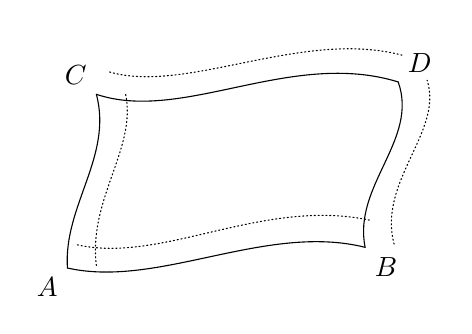
\begin{tikzpicture}[scale=1.05, line cap=round]
  \coordinate (A) at (0,0);
  \coordinate (B) at (3.6,.25);
  \coordinate (C) at (.35,2.1);
  \coordinate (D) at (4.0,2.25);
  \draw (A) .. controls (1.1,-.25) and (2.4,.55) .. (B);
  \draw (C) .. controls (1.4,1.75) and (2.7,2.65) .. (D);
  \draw (A) .. controls (-.05,.75) and (.55,1.35) .. (C);
  \draw (B) .. controls (3.45,1.0) and (4.25,1.55) .. (D);
  \draw[densely dotted] ($(A)+(0.12,.28)$) .. controls (1.15,.05) and (2.35,.85) .. ($(B)+(0.05,.33)$);
  \draw[densely dotted] ($(C)+(0.16,.27)$) .. controls (1.45,2.1) and (2.85,2.9) .. ($(D)+(0.06,.32)$);
  \draw[densely dotted] ($(A)+(0.35,.03)$) .. controls (.25,.85) and (.85,1.45) .. ($(C)+(.35,.02)$);
  \draw[densely dotted] ($(B)+(.35,.04)$) .. controls (3.75,1.05) and (4.55,1.65) .. ($(D)+(.35,.02)$);
  \node[below left] at (A) {$A$};
  \node[below right] at (B) {$B$};
  \node[above left] at (C) {$C$};
  \node[above right] at (D) {$D$};
\end{tikzpicture}
\end{center}

Analytically, if for a given surface the equations of its curves of curvature are
expressed in the form $h=f(x,y,z)$, $k=\phi(x,y,z)$; then the coordinates
$x,y,z$ can

\sourcepage{98}{502}
be expressed each of them as a function of the parameters $h,k$, and we have for
the element of distance between two consecutive points on the surface
\[
dx^2+dy^2+dz^2=A\,dh^2+C\,dk^2,
\]
where $A,C$ are in general each of them a function of $h$ and $k$. The condition
for the divisibility into squares is that the quotient $A\div C$ shall be of the form
function $h\div$ function $k$.

It was shown by M. Bertrand that, in a triple system of orthotomic isothermal
surfaces, each surface possesses the property in question of divisibility into squares
by means of its curves of curvature. But in such a triple system, each surface of
the system is necessarily a quadric; so that the theorem comes to this, that a
quadric surface is, by means of its curves of curvature, divisible into squares. The
analytical verification is at once effected: taking the equation of the surface to be
\[
\frac{X^2}{a}+\frac{Y^2}{b}+\frac{Z^2}{c}=1,
\]
then the expressions for the coordinates in terms of the parameters $h,k$ of a
curve of curvature are
\[
\begin{aligned}
x^2&=\frac{a(a+h)(a+k)}{(a-b)(a-c)},\\
y^2&=\frac{b(b+h)(b+k)}{(b-c)(b-a)},\\
z^2&=\frac{c(c+h)(c+k)}{(c-a)(c-b)},
\end{aligned}
\]
and we have
\[
4(dx^2+dy^2+dz^2)
=(h-k)^2\left\{
\frac{h\,dh^2}{(a+h)(b+h)(c+h)}
-\frac{k\,dk^2}{(a+k)(b+k)(c+k)}
\right\},
\]
so that $A\div C$ is of the required form.

But there is nothing to show that the property is confined to quadric surfaces; and
the question of the determination of the surfaces possessing the property appears to
be one of considerable difficulty, and which has not hitherto been examined.

% ============================================================
% PAPER 503
% ============================================================
\sourcepage{99}{503}
\papersection{503}{On the Surfaces each the Locus of the Vertex of a Cone which Passes through $m$ Given Points and Touches $6-m$ Given Lines.}

\fromjournal{[From the Proceedings of the London Mathematical Society, vol.~\textsc{iv}. (1871--1873), pp.~11--47. Read January 11, 1872.]}

\textsc{I consider} the surfaces, each of them the locus of the vertex of a
(quadri-)cone which passes through $m$ given points and touches $6-m$ given lines;
viz. calling the given points $a,b,c,\ldots$ and the given lines
$\alpha,\beta,\gamma,\ldots$, the surfaces in question are:
\[
\begin{array}{c|c}
\text{surface}&\text{order}\\ \hline
abcdef&4\\
abcde\alpha&8\\
abcd\alpha\beta&16\\
abc\alpha\beta\gamma&24\\
ab\alpha\beta\gamma\delta&24\\
a\alpha\beta\gamma\delta\epsilon&14\\
\alpha\beta\gamma\delta\epsilon\zeta&8
\end{array}
\]

I remark that the orders of these several surfaces are in effect determined by
the investigations of M. Chasles in regard to the conics in space which satisfy
seven conditions. The surface $abcdef$ was long ago considered by M. Chasles, and
it is treated of in my ``Memoir on Quartic Surfaces,'' [445], and in the same Memoir
the surface $\alpha\beta\gamma\delta\epsilon\zeta$ is also referred to: these two
surfaces, and also the surfaces $a\alpha\beta\gamma\delta\epsilon$ and
$ab\alpha\beta\gamma\delta$ are considered by Dr Hierholzer\footnote{I was grieved
to hear of Dr Hierholzer's death last autumn, at Carlsruhe, at the early age of 30.}
in his excellent paper ``Ueber Kegelschnitte im Raume,'' \textit{Math. Annalen},
t.~\textsc{ii}. (1870), pp.~563--586, and to him are due the equations given in the
sequel for the surfaces $abcdef$ and $\alpha\beta\gamma\delta\epsilon\zeta$: the
researches of the present Memoir are in fact a continuation and development of
those in the Memoir last referred to.

\sourcepage{100}{503}
1. We have on the before-mentioned surfaces respectively certain simple or multiple
points, right lines, and curves, as shown in the following Table:

\begin{landscape}
\begin{center}
\small
\setlength{\tabcolsep}{3pt}
\renewcommand{\arraystretch}{1.25}
\begin{tabular}{>{\raggedright\arraybackslash}p{3.6cm}|*{7}{>{\centering\arraybackslash}p{2.6cm}}}
\toprule
& $abcdef,\,4$ & $abcde\alpha,\,8$ & $abcd\alpha\beta,\,16$
& $abc\alpha\beta\gamma,\,24$ & $ab\alpha\beta\gamma\delta,\,24$
& $a\alpha\beta\gamma\delta\epsilon,\,14$
& $\alpha\beta\gamma\delta\epsilon\zeta,\,8$\\
\midrule
Points $a$ & $6\times(2)$ & $5\times(4)$ & $4\times(8)$ & $3\times(8)$ & $2\times(4)$ & $1\times(2)$ & $0$\\
\midrule
$ab$ & $15\times(1),\,C$ & $10\times(2),\,C$ & $6\times(4),\,C$ & $3\times(4),\,C$ & $1\times(2),\,C$ & $0$ & $0$\\
$\alpha$ & $0$ & $1\times(2),\,C$ & $2\times(4),\,C$ & $3\times(8),\,C$ & $4\times(8),\,C$ & $5\times(4),\,C$ & $6\times(2),\,C$\\
$[ab,\alpha,\beta,\gamma]$ & $0$ & $0$ & $0$ & $6\times(4),\,P$ & ${}^{3}3\times(2+2),\,L$ & $0$ & $0$\\
$[\alpha,\beta,\gamma,\delta]$ & $0$ & $0$ & $0$ & $0$ & $2\times(8),\,P$ & $10\times(2),\,L$ & $30\times(1),\,L$\\
$[ab,cd,\alpha,\beta]$ & $0$ & $0$ & $6\times(2),\,P$ & $0$ & $0$ & $0$ & $0$\\
$abc,def$ & $10\times(1),\,P$ & $0$ & $0$ & $0$ & $0$ & $0$ & $0$\\
$abc,de,\alpha$ & $0$ & ${}^{4}10\times(1),\,P$ & $0$ & $0$ & $0$ & $0$ & $0$\\
$abc,\alpha,\beta$ & $0$ & $0$ & ${}^{2}4\times(2+2),\,P$ & $3\times(4),\,P$ & $0$ & $0$ & $0$\\
Cubic $abcdef$ & $1\times(1),\,C$ & $0$ & $0$ & $0$ & $0$ & $0$ & $0$\\
Quadriquadric $\alpha\beta\gamma,\delta\epsilon\zeta$ & $0$ & $0$ & $0$ & $0$ & $0$ & $0$ & ${}^{1}10\times(1),\,L$\\
Excuboquartic $\alpha\beta\gamma,\delta\epsilon,a$ & $0$ & $0$ & $0$ & $0$ & $0$ & ${}^{4}10\times(1),\,L$ & $0$\\
\bottomrule
\end{tabular}
\end{center}
\begin{enumerate}
\item Tangent plane along line is plane $abc$.
\item Tacnodal line, each sheet touched along line by plane $abc$.
\item Tacnodal line, each sheet of surface touched along line by hyperboloid $\alpha\beta\gamma$.
\item Surface touched along line by hyperboloid $\alpha\beta\gamma$.
\end{enumerate}
\end{landscape}

\sourcepage{101}{503}
2. In the Table, the upper margin refers to the surfaces, and the left-hand margin
to the points, lines, and curves situate on these surfaces respectively; the body of
the Table showing the number, and in ( ) the multiplicity, of these points, lines,
and curves in regard to the several surfaces respectively. Thus, points $a$; for
the surface $abcdef$, $6\times(2)$, there are 6 such points, each of them a 2-conical
(ordinary conical) point on the surface: so $abcde\alpha$, $5\times(4)$, there are
5 such points, each a 4-conical point on the surface (viz. instead of the tangent
plane there is a quartic cone); and so on. Similarly, lines $ab$ (viz. these are the
lines joining two points $a,b$); for the surface $abcdef$, $15\times(1)$, there are
15 such lines, each a simple line on the surface; surface $abcde\alpha$,
$10\times(2)$, there are 10 such lines, each a double (ordinary nodal) line on the
surface; and so on. We have in two places the multiplicity $(2+2)$, which refers
to a tacnodal line, as presently explained. The corner letters $C,P,L$ denote
respectively proper cone, plane-pair, and line-pair, as afterwards explained.

3. The lines and curves referred to in the left-hand margin are:
\begin{enumerate}
\item $ab$, line joining the points $a$ and $b$.
\item $\alpha$, line $\alpha$.
\item $[ab,\alpha,\beta,\gamma]$, pair of lines meeting each of the four lines, or say
the tractors of the four lines $ab,\alpha,\beta,\gamma$. As regards the surface
$ab\alpha\beta\gamma\delta$, the multiplicity is given as $(2+2)$, viz. the line is
(not an ordinary nodal, but) a tacnodal line, each sheet touching along the whole
line the hyperboloid $\alpha\beta\gamma$.
\item $[\alpha,\beta,\gamma,\delta]$, tractors of the four lines
$\alpha,\beta,\gamma,\delta$.
\item $[ab,cd,\alpha,\beta]$ tractors of the four lines $ab,cd,\alpha,\beta$.
\item $abc,def$, line of intersection of the planes $abc$ and $def$.
\item $abc,de,\alpha$, line in the plane $abc$ joining the intersections of this plane
by the lines $de$ and $\alpha$ respectively.
\item $abc,\alpha,\beta$, line in the plane $abc$ joining the intersections of this
plane by the lines $\alpha$ and $\beta$ respectively. As regards the surface
$abcd\alpha\beta$, the multiplicity is given as $(2+2)$, viz. each line is (not an
ordinary nodal, but) a tacnodal line, each sheet touching along the whole line the
plane $abc$.
\item Cubic $abcdef$, cubic curve through the six points $a,b,c,d,e,f$, common
intersection of the cones each having its vertex at one of the points and passing
through the other five.
\item Quadriquadric $\alpha\beta\gamma,\delta\epsilon\zeta$, intersection of the
quadric surfaces $\alpha\beta\gamma$ and $\delta\epsilon\zeta$ that is, the quadric
surfaces through the lines $\alpha,\beta,\gamma$ and
$\delta,\epsilon,\zeta$ respectively.
\item Excuboquartic $\alpha\beta\gamma,\delta\epsilon,a$, quartic curve generated as
follows: viz. taking any line whatever which meets the lines $\alpha,\beta,\gamma$
(or say any generating line of the quadric $\alpha\beta\gamma$), the plane through
this line and the point $a$ meets the lines $\delta,\epsilon$ in two points respectively;
and the line joining these meets the generating line in a point having for its locus
the excuboquartic curve in question (theory further considered in the sequel).
\end{enumerate}

\sourcepage{102}{503}
\subsection*{Special forms of (Quadri-)Cones.}

4. We have to consider the special forms of (quadri-)cones; these are: 1\textdegree.
The sharp-cone, or plane-pair; that is, a pair of two planes, intersecting in a line
called the axis, the vertex being in this case an indeterminate point on the axis.
Observe that a plane-pair passes through a given point when either of its planes
passes through such point; it touches a given line when its axis meets the given
line. 2\textdegree. The flat-cone, or line-pair; viz. this is a pair of intersecting
lines, their point of intersection being the vertex of the line-pair, and the plane of
the two lines being the diametral of the line-pair. Observe that the line-pair passes
through a given point when its diametral passes through such point; it touches a
given line when either of its lines meets the given line. 3\textdegree. There is a
third kind, the line-pair-plane; viz. the two planes of the plane-pair may come to
coincide, retaining, however, a definite line of intersection, or axis: or again, the two
lines of a line-pair may come to coincide, retaining a definite plane or diametral;
that is, in either case we have a plane passing through a line; and which is to be
considered indifferently as two coincident planes intersecting in the line, or as two
coincident lines lying in the plane. But there is not, in the present Memoir, any
occasion to consider this third kind of special cone.

The letters $C,P,L$ in the Table denote that the cone is a (proper) cone, plane-pair,
or line-pair, as the case may be.

\subsection*{Singular Lines and Curves on the Surfaces.}

5. We may establish \textit{a priori} the existence, and even to some extent the
multiplicity, of the several lines and curves on the surfaces
$abcdef,\ldots,\alpha\beta\gamma\delta\epsilon\zeta$. Thus:

1\textdegree. Lines $ab$: take for the vertex of the cone a point at pleasure on the
line $ab$; the cone passing through $b$ will \textit{ipso facto} pass through $a$; and
the conditions are thus that the cone shall pass through $b$ and satisfy four other
conditions---in all, five conditions: and there is thus a cone with the point in
question as vertex; that is, the line $ab$ is situate on the surface. Moreover, for
the surfaces $abcdef$, $abcde\alpha$, $abcd\alpha\beta$, $abc\alpha\beta\gamma$,
$ab\alpha\beta\gamma\delta$ respectively, for a given position of the vertex on the
line $ab$, the number of cones is $1,2,4,4,2$ respectively: and these are the
multiplicities of the line $ab$ on the several surfaces respectively.

2\textdegree. Lines $\alpha$: take for the vertex of the cone a point at pleasure on
the line $\alpha$; then the cone \textit{ipso facto} touches the line $\alpha$, and
there are only five other conditions to be satisfied; that is, we have a cone with
the vertex in question; or the line $\alpha$ is situate on the surface. Moreover, for
the surfaces $abcde\alpha$, $abcd\alpha\beta$, $abc\alpha\beta\gamma$,
$ab\alpha\beta\gamma\delta$, $a\alpha\beta\gamma\delta\epsilon$,
$\alpha\beta\gamma\delta\epsilon\zeta$ respectively, the number of cones is
$1,2,4,4,2,1$ respectively: and it may be seen that the multiplicities of the line
$\alpha$ are the doubles of these numbers, or are $=2,4,8,8,4,2$ for the several
surfaces respectively.

\sourcepage{103}{503}
3\textdegree. Lines $[ab,\alpha,\beta,\gamma]$: taking the vertex in one of these
tractors, the cone cannot be a proper cone, but (if it exist) it must be either a
line-pair having the tractor for one of its lines, or else a plane-pair having the
tractor for its axis. The two cases are:

Surface $abc\alpha\beta\gamma$. Cone is a plane-pair, the two planes intersecting
in the tractor, and passing, the one of them through the points $a,b$, the other
through the point $c$. The vertex being an indeterminate point on the tractor, the
tractor is situate on the surface.

Surface $ab\alpha\beta\gamma\delta$. Cone is a line-pair, one line being the
tractor, the other a line drawn in the plane of the tractor and $ab$ to meet
$\delta$, and which meets the tractor in an arbitrary point thereof: the tractor is
thus a line on the surface.

4\textdegree. Lines $[\alpha,\beta,\gamma,\delta]$: taking the vertex in one of
these tractors, then, as in the last case, the cone is either a line-pair having the
tractor for one of its lines or a plane-pair having the tractor for its axis. The three
cases are:

Surface $ab\alpha\beta\gamma\delta$. Cone is a plane-pair, the two planes
intersecting in the tractor and passing through the points $a,b$ respectively.

Surface $a\alpha\beta\gamma\delta\epsilon$. Cone is a line-pair, one line being
the tractor, the other a line in the plane of the tractor and $\alpha$, meeting the
line $\epsilon$ and meeting the tractor in an indeterminate point.

Surface $\alpha\beta\gamma\delta\epsilon\zeta$. Cone is a line-pair, one line
being the tractor, the other a line drawn from an indeterminate point of the tractor
to meet the lines $\epsilon$ and $\zeta$.

5\textdegree. Lines $[ab,cd,\alpha,\beta]$. Cone is a plane-pair, the two planes
intersecting in the tractor, and passing through the points $a,b$ and the points
$c,d$ respectively.

6\textdegree. Line $abc,def$. Cone is a plane-pair, consisting of the two planes
$abc$ and $def$.

7\textdegree. Line $abc,de,\alpha$. Cone is a plane-pair, the two planes intersecting
in the line; one plane being $abc$, the other a plane through the line $de$.

8\textdegree. Line $abc,\alpha,\beta$. There are two cases:

Surface $abcd\alpha\beta$. Cone is a plane-pair, the two planes intersecting in
the line; the one being $abc$, and the other passing through the point $d$.

Surface $abc\alpha\beta\gamma$. Cone is a line-pair; one line being
$abc,\alpha,\beta$, the other a line in the plane $abc$ meeting the line $\delta$,
and meeting the line $abc,\alpha,\beta$ in an indeterminate point.

9\textdegree. Cubic $abcdef$. Each point of the cubic is the vertex of a proper
cone passing through the cubic, and therefore through the six points; that is, the
cubic is a line on the surface $abcdef$.

10\textdegree. Quadriquadric $\alpha\beta\gamma,\delta\epsilon\zeta$. Cone is a
line-pair; viz. it is composed of the lines drawn from any point of the curve, one
of them to meet the lines $\alpha,\beta,\gamma$, and the other to meet the lines
$\delta,\epsilon,\zeta$.

11\textdegree. Excuboquartic $\alpha\beta\gamma,\delta\epsilon,a$. Cone is a
line-pair; the two lines being, one of them a line at pleasure meeting
$\alpha,\beta,\gamma$, the other the line which, in the plane of the other line and
the point $a$, meets the lines $\delta,\epsilon$.

\sourcepage{104}{503}
\subsection*{Mode of obtaining the several Equations: Notations and Formulas.}

6. The equations of the several surfaces are obtained by taking as centre of projection
an assumed position of the vertex, and projecting everything upon an arbitrary plane;
the projections of the given points and lines are points and lines in the arbitrary
plane, and the section of the cone by this plane is a conic; the equation of the
surface is thus obtained as the condition that there shall be a conic passing through
$m$ given points and touching $6-m$ given lines.

7. We take as current coordinates $(X,Y,Z,W)$, or when plane-coordinates are
employed $(\xi,\eta,\zeta,\omega)$: the coordinates of the vertex are throughout
represented by $(x,y,z,w)$; but in explanations \&c., these are also used as current
coordinates. The plane of projection is taken to be $W=0$. The coordinates of the
given points $a$, \&c., are taken to be $(x_a,y_a,z_a,w_a)$, \&c. There is no
confusion occasioned by so doing, and I retain the ordinary letters $(a,b,c,f,g,h)$
for the six coordinates of a line, it being understood that these letters so used have
no reference whatever to the given points $a,b$, \&c.; viz. the coordinates of the
given lines $\alpha$, \&c., are
$(a_\alpha,b_\alpha,c_\alpha,f_\alpha,g_\alpha,h_\alpha)$, \&c.; there is sometimes
occasion to consider the coordinates of other lines $ab$, \&c., but the notation will
always be explained.

8. I write $l,m,n,p,q,r$ for the coordinates of the line joining the vertex
$(x,y,z,w)$ with a point $(x',y',z',w')$; viz.
\[
l=yz'-y'z,\quad p=xw'-x'w,\qquad
m=zx'-z'x,\quad q=yw'-y'w,
\]
\[
n=xy'-x'y,\quad r=zw'-z'w,
\]
($l_a=yz_a-y_az$, \&c., this being explained when necessary); and also
\[
\begin{aligned}
P&=\phantom{-}hy-gz+aw,\\
Q&=-hx+fz+bw,\\
R&=\phantom{-}gx-fy+cw,\\
S&=-ax-by-cz,
\end{aligned}
\]
($P_\alpha=h_\alpha y-g_\alpha z+a_\alpha w$, \&c., this being explained when
necessary).

This being so, then projecting from the vertex $(x,y,z,w)$, say on the plane $W=0$,
the $x,y,z$ coordinates of the projection of a point $a$ are as
$p_a:q_a:r_a$ ($p_a=xw_a-x_aw$, \&c.); and the equation of the projection of a line
$\alpha$ is
\[
P_\alpha X+Q_\alpha Y+R_\alpha Z=0
\]
($P_\alpha=h_\alpha y-g_\alpha z+a_\alpha w$, \&c.). We thus have, in the projection
on the plane $W=0$, the $m$ points and $6-m$ lines situate in and touched by the conic.

\sourcepage{105}{503}
The following notations and formulae are convenient:

9. $\p_{abc}=0$ is the equation of the plane through the points $a,b,c$; viz.
\[
\p_{abc}=\Det{
x&y&z&w\\
x_a&y_a&z_a&w_a\\
x_b&y_b&z_b&w_b\\
x_c&y_c&z_c&w_c}.
\]
Of course $\p_{bac}=-\p_{abc}$, \&c. Observe that here, and in the notations which
follow, the letter $\p$ is used as referring to the coordinates $(x,y,z,w)$, and that
the index of $\p$ ($=1$ when no index is expressed) shows the degree in these
coordinates.

10. $\p_{a\alpha}=0$ is the equation of the plane through the point $a$ and the
line $\alpha$; viz. $\p_{a\alpha}$ is the foregoing determinant, if for a moment
$b,c$ are any two points on the line $\alpha$; or, what is the same thing,
\[
\p_{a\alpha}=P_\alpha x_a+Q_\alpha y_a+R_\alpha z_a+S_\alpha w_a,
\]
where
\[
\begin{aligned}
P_\alpha&=\phantom{-}h x_a-g z_a+a w_a,\\
Q_\alpha&=-h x_a+f z_a+b w_a,\\
R_\alpha&=\phantom{-}g x_a-f y_a+c w_a,\\
S_\alpha&=-a x_a-b y_a-c z_a.
\end{aligned}
\]
and $(a,b,c,f,g,h)$ are the coordinates of the line $\alpha$: observe that
$\p_{a\alpha}=\p_{\alpha a}$.

11. $\p^2_{\alpha\beta\gamma}=0$ is the equation of the quadric surface through
the lines $\alpha,\beta,\gamma$; viz. we have
\[
\begin{aligned}
\p^2_{\alpha\beta\gamma}
&=(agh)x^2+(bhf)y^2+(cfg)z^2+(abc)w^2\\
&\quad+[(abg)-(cah)]xw+[(bch)-(abf)]yw+[(caf)-(bcg)]zw\\
&\quad+[(bcf)+(ach)]yz+[(cag)+(bfh)]zx+[(abh)+(bgh)]xy,
\end{aligned}
\]
where
\[
agh=\Det{a_\alpha&g_\alpha&h_\alpha\\
a_\beta&g_\beta&h_\beta\\
a_\gamma&g_\gamma&h_\gamma},
\]
\&c. $(a_\alpha,b_\alpha,c_\alpha,f_\alpha,g_\alpha,h_\alpha)$,
$(a_\beta,\ldots)$, $(a_\gamma,\ldots)$ being the coordinates of the given lines
$\alpha,\beta,\gamma$. Observe that
$\p^2_{\beta\alpha\gamma}=-\p^2_{\alpha\beta\gamma}$, \&c.

\sourcepage{106}{503}
12. It is to be noticed that, writing
\[
P=hy-gz+aw,\quad Q=-hx+fz+bw,\quad R=gx-fy+cw,\quad S=-ax-by-cz,
\]
viz. $P_\alpha=h_\alpha y-g_\alpha z+a_\alpha w$, \&c., then that we have identically
\[
\Det{
\lambda&\mu&\nu&\rho\\
P_\alpha&Q_\alpha&R_\alpha&S_\alpha\\
P_\beta&Q_\beta&R_\beta&S_\beta\\
P_\gamma&Q_\gamma&R_\gamma&S_\gamma}
=-(\lambda x+\mu y+\nu z+\rho w)\,\p^2_{\alpha\beta\gamma},
\]
and further that we have identically
\[
-\p^2_{\alpha\beta\gamma}
=L_{\alpha\beta}P_\gamma+M_{\alpha\beta}Q_\gamma
+N_{\alpha\beta}R_\gamma+\Omega_{\alpha\beta}S_\gamma,
\]
where
\[
\begin{aligned}
L&=(af'-a'f)x+(bf'-b'f)y+(cf'-c'f)z-(bc'-b'c)w,\\
M&=(ag'-a'g)x+(bg'-b'g)y+(cg'-c'g)z-(ca'-c'a)w,\\
N&=(ah'-a'h)x+(bh'-b'h)y+(ch'-c'h)z-(ab'-a'b)w,\\
\Omega&=(gh'-g'h)x+(hf'-h'f)y+(fg'-f'g)z\\
&\quad+(af'-a'f+bg'-b'g+ch'-c'h)w;
\end{aligned}
\]
and $L_{\alpha\beta}$, \&c. are the values of $L$, \&c. on substituting therein
$(a_\alpha,\ldots)$ and $(a_\beta,\ldots)$ for the unaccented and accented letters
respectively.

13. Observe that we have
\[
\begin{aligned}
L+(a'f+b'g+c'h)x&=-c'Q+b'R-f'S,\\
M+(a'f+b'g+c'h)y&= c'P-a'R-g'S,\\
N+(a'f+b'g+c'h)z&=-b'P+a'Q-h'S,\\
\Omega+(a'f+b'g+c'h)w&=f'P+g'Q+h'R,
\end{aligned}
\]
and similarly
\[
\begin{aligned}
-L+(af'+bg'+ch')x&=-cQ'+bR'-fS',\\
-M+(af'+bg'+ch')y&= cP'-aR'-gS',\\
-N+(af'+bg'+ch')z&=-bP'+aQ'-hS',\\
-\Omega+(af'+bg'+ch')w&=fP'+gQ'+hR'.
\end{aligned}
\]
whence also
\[
\begin{aligned}
h'M-g'N+a'\Omega&=-(a'f+b'g+c'h)P',\\
-h'L+f'N+b'\Omega&=-(a'f+b'g+c'h)Q',\\
g'L-f'M+c'\Omega&=-(a'f+b'g+c'h)R',\\
-a'L-b'M-c'N&=-(a'f+b'g+c'h)S',
\end{aligned}
\]
\sourcepage{107}{503}
and
\[
\begin{aligned}
hM-gN+a\Omega&=(af'+bg'+ch')P,\\
-hL+fN+b\Omega&=(af'+bg'+ch')Q,\\
gL-fM+c\Omega&=(af'+bg'+ch')R,\\
-aL-bM-cN&=(af'+bg'+ch')S.
\end{aligned}
\]

14. $\p^3_{a.\alpha\beta.\gamma\delta}=0$ is the equation of the cubic surface
through the lines $\alpha,\beta,\gamma,\delta$ and $a\alpha\beta$, $a\gamma\delta$
(viz. $a\alpha\beta$ is the line from $a$ to meet $\alpha,\beta$, and so
$a\gamma\delta$ is the line from $a$ to meet $\gamma,\delta$). Observe that the
conditions which determine this cubic surface thus are that the cubic shall pass
through
\[
\begin{gathered}
a;\ \hbox{the points of }a\alpha\beta\hbox{ on }\alpha\hbox{ and }\beta
\hbox{ respectively, 3 other points on }\alpha,3\hbox{ on }\beta,\\
\hbox{and 1 on }a\alpha\beta;
\end{gathered}
\]
also the points of $a\gamma\delta$ on $\gamma$ and $\delta$ respectively, 3 other
points on $\gamma$, 3 on $\delta$, and 1 on $a\gamma\delta$; in all, $1+9+9=19$
points; viz. the conditions completely determine the surface.

15. We have
\[
\p^3_{a.\alpha\beta.\gamma\delta}
=\Det{
x&y&z&w\\
x_a&y_a&z_a&w_a\\
L_{\alpha\beta}&M_{\alpha\beta}&N_{\alpha\beta}&\Omega_{\alpha\beta}\\
L_{\gamma\delta}&M_{\gamma\delta}&N_{\gamma\delta}&\Omega_{\gamma\delta}},
\]
viz. this determinant, equated to zero, gives the equation of the surface.

To prove this, take as before the unaccented letters $(a,b,c,f,g,h)$ to refer to
the line $\alpha$, and the letters with one, two, and three accents to refer to the
lines $\beta,\gamma,\delta$ respectively; write also $L,M,N,\Omega$ and
$L',M',N',\Omega'$ for $L_{\alpha\beta}$, \&c., and $L_{\gamma\delta}$, \&c.,
respectively. Referring to the foregoing expressions for $L,M,N,\Omega$, and observing
that for a point on the line $\alpha$, the values of $P,Q,R,S$ are each $=0$, then
for such a point we have
\[
L+(a'f+b'g+c'h)x=0,\quad \&c.,
\]
that is, $L:M:N:\Omega=x:y:z:w$, and these values satisfy the equation of the
surface, which is thus a surface passing through the line $\alpha$; and similarly it
passes through the lines $\beta,\gamma,\delta$.

To show that the surface passes through the line $a\alpha\beta$, take the coordinates
of the point $a$ to be $0,0,0,1$; then the line $a\alpha\beta$ is given as the
intersection of the planes $ax+by+cz=0$ and $a'x+b'y+c'z=0$, that is, $S=0$ and
$S'=0$. And the equation of the surface, writing therein $x_a,y_a,z_a,w_a=0,0,0,1$,
becomes
\[
\Det{x&y&z\\ L&M&N\\ L'&M'&N'}=0,
\]
\sourcepage{108}{503}
or, as this may be written,
\[
\Det{
S&S'&z\\
aL+bM+cN&a'L+b'M+c'N&N\\
aL'+bM'+cN'&a'L'+b'M'+c'N'&N'}=0.
\]
For a point on the line $a\alpha\beta$, this is
\[
\Det{
aL+bM+cN&a'L+b'M+c'N\\
aL'+bM'+cN'&a'L'+b'M'+c'N'}=0.
\]
But in the equations
\[
-a'L-b'M-c'N=-(a'f+b'g+c'h)S',
\quad
-aL-bM-cN=(af'+bg'+ch')S,
\]
writing $S=0$ and $S'=0$, we have
$aL+bM+cN=0$ and $a'L+b'M+c'N=0$, and the equation is satisfied; that is, the
surface passes through the line $a\alpha\beta$, and similarly it passes through the
line $a\gamma\delta$.

\subsection*{Surface $abcdef$.}

16. The equation may be written
\[
\p_{abe}\p_{cde}\p_{acf}\p_{dbf}
-\p_{abf}\p_{cdf}\p_{ace}\p_{dbe}=0,
\]
where $\p_{abe}=0$ is the equation of the plane through the points $a,b,e$; and the
like for the other symbols. The form is one out of 45 like forms, depending on the
partitionment
\[
\begin{matrix}
ab.cd\\
ac.db\\
ad.bc
\end{matrix}\Bigg\}(ef),
\]
of the six letters.

17. Investigation. In the projection, the six points $(p_a,q_a,r_a)$ are situate on
a conic; the condition for this is
\[
\Det{p^2&q^2&r^2&qr&rp&pq}_{a,b,c,d,e,f}=0,
\]
where the left-hand side represents the determinant obtained by writing successively
$(p_a,q_a,r_a)$, \&c., for $(p,q,r)$. The equation in question may be written
\[
abe.cde.acf.dbf-abf.cdf.ace.dbe=0;
\]
where
\[
abe=\Det{p_a&q_a&r_a\\p_b&q_b&r_b\\p_e&q_e&r_e},\quad \&c.
\]
and substituting for $p_a,\ldots$, their values, we have $abe=w^2\p_{abe}$, whence
the foregoing result.
\surf{abcdef}

\sourcepage{109}{503}
18. Singularities. The form of the equation shows at once that\footnote{Of course,
as regards the present surface and the other surfaces for which the equation is given
in an unsymmetrical form, the conclusion obtained in regard to any point or line of
the surface applies to every point or line of the same kind. Thus $ab$ being a simple
line, we have also $ad$ a simple line, although the equation, as written down, does
not put this in evidence.}
\begin{enumerate}
\item[(0)]\footnote{The bracketed numbers refer to the lines of the Table.} The
point $a$ is a 2-conical point; in fact, for this point we have
$\p_{abe}=0$, $\p_{acf}=0$, $\p_{abf}=0$, $\p_{ace}=0$.
\item[(1)] The line $ab$ a simple line; in fact, for any point of this line we have
$\p_{abe}=0$, $\p_{abf}=0$.
\item[(2)] The line $abe.cdf$ a simple line; in fact, for any point of this line we
have $\p_{abe}=0$, $\p_{cdf}=0$.
\item[(9)] To show analytically that the cubic curve $abcdef$ is a line on the
surface, observe that the equation of the surface is satisfied if we have simultaneously
($\lambda$ being arbitrary)
\[
\p_{abe}\p_{acf}-\lambda\p_{abf}\p_{ace}=0,\qquad
\lambda\p_{cde}\p_{dbf}-\p_{cdf}\p_{dbe}=0.
\]
\end{enumerate}
The first of these equations is a cone, vertex $a$, which passes through the points
$b,e,c,f$, and which, if $\lambda$ is properly determined, will pass through the point
$d$; the second is a cone, vertex $d$, which passes through the points $b,e,c,f$,
and which, if $\lambda$ is properly determined, will pass through the point $a$; the
two determinations of $\lambda$ are
\[
dabe.dacf-\lambda\,dabf.dace=0,\qquad
\lambda\,acde.adbf-acdf.adbe=0;
\]
giving the same value of $\lambda$; and the equations then represent cones, the first
having $a$ for its vertex, and passing through $d,b,e,c,f$; the second having $d$
for its vertex, and passing through $a,b,e,c,f$; the two intersect in the line $ad$,
and in the cubic curve $abcdef$, which is thus a curve on the surface.

\subsection*{Surface $abcde\alpha$.}

19. The equation may be written
\[
\bigl(\p_{abe}\p_{cde}\p^2_{\alpha.ac.db}
-\p_{ace}\p_{dbe}\p^2_{\alpha.ab.cd}\bigr)^2
+4\p_{abe}\p_{cde}\p_{ace}\p_{dbe}\p_{abc}\p_{dbc}\p_{a\alpha}\p_{d\alpha}=0,
\]
or, what is the same thing,
\[
\begin{aligned}
&\bigl(\p_{abe}\p_{cde}\p^2_{\alpha.ac.db}
+\p_{ace}\p_{dbe}\p^2_{\alpha.ab.cd}\bigr)^2\\
&\qquad+4\p_{abe}\p_{cde}\p_{ace}\p_{dbe}\p_{bad}\p_{cad}\p_{b\alpha}\p_{c\alpha}=0,
\end{aligned}
\]
(the equivalence of the two depending on the identity
\[
-\p^2_{\alpha.ab.cd}\p^2_{\alpha.ac.db}
+\p_{abc}\p_{dbc}\p_{a\alpha}\p_{d\alpha}
-\p_{bad}\p_{cad}\p_{b\alpha}\p_{c\alpha}=0)
\]
\sourcepage{110}{503}
where, as before, $\p_{abe}=0$ is the equation of the plane through the points
$a,b,e$; $\p^2_{\alpha.ac.db}=0$ the equation of the quadric surface through the
lines $\alpha,ac,db$; and $\p_{a\alpha}=0$ the equation of the plane through the
point $a$ and the line $\alpha$.

The above forms are 2 out of 30 like forms, as appears by the partitionment
\[
\left\{
\begin{matrix}
ab,&cd\\
ac,&db\\
ad,&bc
\end{matrix}
\right\}e\alpha.
\]

20. Investigation. In the projection, the equation of the conic through the five
points may be written
\[
\left|\begin{array}{c}
(X,Y,Z)^2\\
(p,q,r)^2
\end{array}\right|=0,
\]
where the symbol denotes a determinant the last five lines of which are obtained by
giving to $(p,q,r)$ the suffixes $a,b,c,d,e$ respectively. This is at once transformed
into
\[
abe.cde.ac\Delta.db\Delta-ace.dbe.ab\Delta.cd\Delta=0,
\]
or, what is the same thing,
\[
\p_{abe}\p_{cde}.ac\Delta.db\Delta-\p_{ace}\p_{dbe}.ab\Delta.cd\Delta=0,
\]
or say,
\[
\p_{abe}\p_{cde}(A''X+B''Y+C''Z)(A'''X+B'''Y+C'''Z)
-\p_{ace}\p_{dbe}(AX+BY+CZ)(A'X+B'Y+C'Z),
\]
where $\p_{abe}$, \&c. signify as before, and
\[
AX+BY+CZ=\Det{X&Y&Z\\p_a&q_a&r_a\\p_b&q_b&r_b},
\]
and so for $A'X+B'Y+C'Z$, \&c., the suffixes for $A',B',C'$ being $(c,d)$, and
those for $A'',B'',C''$ and $A''',B''',C'''$ being $(a,c)$ and $(d,b)$ respectively.

21. Passing to the reciprocal equation, and making the conic touch the line $\alpha$,
we obtain the equation of the surface in the form
\[
\begin{aligned}
&\left\{\p_{abe}\p_{cde}
\Det{P_\alpha&Q_\alpha&R_\alpha\\ A''&B''&C''\\A'''&B'''&C'''}
-\p_{ace}\p_{dbe}
\Det{P_\alpha&Q_\alpha&R_\alpha\\ A&B&C\\A'&B'&C'}\right\}^2\\
&\quad+4\p_{ace}\p_{dbe}\p_{abe}\p_{cde}
\Det{P_\alpha&Q_\alpha&R_\alpha\\ A&B&C\\A''&B''&C''}
\Det{P_\alpha&Q_\alpha&R_\alpha\\ A'&B'&C'\\A'''&B'''&C'''}=0,
\end{aligned}
\]
\sourcepage{111}{503}
where $P_\alpha=h_\alpha y-g_\alpha z+a_\alpha w=0$; or in the equivalent form
wherein we have in the first term $+$ instead of $-$, and in the second term the
determinants
\[
\Det{P_\alpha&Q_\alpha&R_\alpha\\A&B&C\\A'''&B'''&C'''},
\qquad
\Det{P_\alpha&Q_\alpha&R_\alpha\\A'&B'&C'\\A''&B''&C''}.
\]

22. \{The question, in fact, is to find the reciprocal of the form
\[
\lambda(ax+by+cz)(a'x+b'y+c'z)
-\mu(a''x+b''y+c''z)(a'''x+b'''y+c'''z)=0;
\]
taking $\xi,\eta,\zeta$ for the reciprocal variables, the coefficient of $\xi^2$ is
\[
\{\lambda(bc'+b'c)-\mu(b''c'''+b'''c'')\}^2
-(2\lambda bb'-2\mu b''b''')(2\lambda cc'-2\mu c''c'''),
\]
viz. this is
\[
\lambda^2(bc'-b'c)^2+\mu^2(b''c'''-b'''c'')^2
+2\lambda\mu\{2bb'c''c'''+2b''b'''cc'-(bc'+b'c)(b''c'''+b'''c'')\},
\]
or, as it may be written,
\[
\{\lambda(bc'-b'c)\pm\mu(b''c'''-b'''c'')\}^2
+2\lambda\mu
\begin{pmatrix}
2bb'c''c'''+2b''b'''cc'\\
\mp(bc-b'c)(b''c'''-b'''c'')\\
-(bc'+b'c)(b''c'''+b'''c'')
\end{pmatrix}.
\]
Taking the upper signs, this is
\[
\{\lambda(bc'-b'c)+\mu(b''c'''-b'''c'')\}^2
+4\lambda\mu
\begin{pmatrix}
bb'c''c'''+b''b'''cc'\\
-bc'b''c'''-b'cb'''c''
\end{pmatrix};
\]
viz. the term in $\lambda\mu$ is
\[
=+4\lambda\mu(bc'''-b'''c)(b'c''-b''c').
\]
Taking the lower signs, it is
\[
\{\lambda(bc'-b'c)-\mu(b''c'''-b'''c'')\}^2
+4\lambda\mu
\begin{pmatrix}
bb'c''c'''+b''b'''cc'\\
-bc'b'''c''-b'cb''c'''
\end{pmatrix};
\]
viz. the term in $\lambda\mu$ is
\[
4\lambda\mu(bc''-b''c)(b'c'''-b'''c');
\]
and it is thence easy to infer the forms of the other coefficients, and to obtain
the reciprocal equation in the two equivalent forms
\[
\begin{aligned}
&\{\lambda\Det{\xi&\eta&\zeta\\a&b&c\\a'&b'&c'}
+\mu\Det{\xi&\eta&\zeta\\a''&b''&c''\\a'''&b'''&c'''}\}^2\\
&\quad+4\lambda\mu
\Det{\xi&\eta&\zeta\\a&b&c\\a'''&b'''&c'''}
\Det{\xi&\eta&\zeta\\a'&b'&c'\\a''&b''&c''}=0,
\end{aligned}
\]
\[
\begin{aligned}
&\{\lambda\Det{\xi&\eta&\zeta\\a&b&c\\a'&b'&c'}
-\mu\Det{\xi&\eta&\zeta\\a''&b''&c''\\a'''&b'''&c'''}\}^2\\
&\quad+4\lambda\mu
\Det{\xi&\eta&\zeta\\a&b&c\\a''&b''&c''}
\Det{\xi&\eta&\zeta\\a'&b'&c'\\a'''&b'''&c'''}=0,
\end{aligned}
\]
which are the required auxiliary formulae.\}
\surf{abcde\alpha}

\sourcepage{112}{503}
23. To reduce the foregoing result, we have
\[
A,B,C=
\Det{xw_a-wx_a&yw_a-wy_a&zw_a-wz_a\\
xw_b-wx_b&yw_b-wy_b&zw_b-wz_b}
\]
proportional to the three determinants which contain $w$, of the set
\[
\begin{matrix}
x&y&z&w\\
x_a&y_a&z_a&w_a\\
x_b&y_b&z_b&w_b
\end{matrix},
\qquad
\hbox{viz.}\quad
A=w\Det{y&z&w\\y_a&z_a&w_a\\y_b&z_b&w_b},
\]
and similarly $A',B',C'$ are proportional to the three determinants which contain
$w$, of the set
\[
\begin{matrix}
x&y&z&w\\
x_c&y_c&z_c&w_c\\
x_d&y_d&z_d&w_d
\end{matrix},
\qquad
\hbox{viz.}\quad
A'=w\Det{y&z&w\\y_c&z_c&w_c\\y_d&z_d&w_d},
\]
\&c. Hence, omitting the factor $w$, and writing $(a,b,c,f,g,h)$ and
$(a',b',c',f',g',h')$ for the coordinates of the lines $ab$ and $cd$ respectively,
we have
\[
\begin{aligned}
A&=hy-gz+aw,& A'&=h'y-g'z+a'w,\\
B&=-hx+fz+bw,& B'&=-h'x+f'z+b'w,\\
C&=gx-fy+cw,& C'&=g'x-f'y+c'w;
\end{aligned}
\]
and thence
\[
BC'-B'C=\Omega x-Lw,\quad CA'-C'A=\Omega y-Mw,\quad AB'-A'B=\Omega z-Nw,
\]
where
\[
\begin{aligned}
L&=(af'-a'f)x+(bf'-b'f)y+(cf'-c'f)z-(bc'-b'c)w,\\
M&=(ag'-a'g)x+(bg'-b'g)y+(cg'-c'g)z-(ca'-c'a)w,\\
N&=(ah'-a'h)x+(bh'-b'h)y+(ch'-c'h)z-(ab'-a'b)w,\\
\Omega&=(gh'-g'h)x+(hf'-h'f)y+(fg'-f'g)z\\
&\quad-(af'-a'f+bg'-b'g+ch'-c'h)w;
\end{aligned}
\]
and consequently
\[
\begin{aligned}
\Det{P_\alpha&Q_\alpha&R_\alpha\\A&B&C\\A'&B'&C'}
&=\Omega(xP_\alpha+yQ_\alpha+zR_\alpha)
-w(LP_\alpha+MQ_\alpha+NR_\alpha)\\
&=-w(LP_\alpha+MQ_\alpha+NR_\alpha+\Omega S_\alpha),
\end{aligned}
\]
or omitting the factor $-w$, say it is
$LP_\alpha+MQ_\alpha+NR_\alpha+\Omega S_\alpha$, viz. this is
$=\p^2_{\alpha.ab.cd}$.
\surf{abcde\alpha}

\sourcepage{113}{503}
We have similarly
\[
\Det{P_\alpha&Q_\alpha&R_\alpha\\A''&B''&C''\\A'''&B'''&C'''}
\]
taken to be $=\p^2_{\alpha.ac.db}$.

24. We have in like manner the other two determinants
\[
\Det{P_\alpha&Q_\alpha&R_\alpha\\A&B&C\\A''&B''&C''},
\qquad
\Det{P_\alpha&Q_\alpha&R_\alpha\\A'&B'&C'\\A'''&B'''&C'''}
\]
taken to be $=\p^2_{\alpha.ab.ac}$ and $\p^2_{\alpha.cd.db}$ respectively.
But we have
\[
\p^2_{\alpha.ab.ac}=\p_{a\alpha}\p_{abc},
\]
(viz. geometrically the hyperboloid through the lines $\alpha,ab,ac$ breaks up
into the plane $\p_{a\alpha}$ through the line $\alpha$ and point $a$, and the
plane $\p_{abc}$ through the points $a,b,c$).

And similarly
\[
\p^2_{\alpha.cd.db}=-\p^2_{\alpha.dc.db}
=+\p^2_{\alpha.db.dc}=\p_{d\alpha}\p_{dbc};
\]
whence, substituting for the several determinants, we have the foregoing equation
of the surface.

25. Singularities. The form of the equation shows that
\begin{enumerate}
\item[(0)] The point $a$ is a 4-conical point: in fact, for this point we have
$\p_{abe}=0$, $\p^2_{\alpha.ac.db}=0$, $\p_{ace}=0$,
$\p^2_{\alpha.ab.cd}=0$.
\item[(1)] The line $ab$ is a double line: in fact, for any point of the line we
have $\p_{abe}=0$, $\p^2_{\alpha.ab.cd}=0$, $\p_{abc}=0$.
\item[(2)] The line $\alpha$ is a double line: in fact, for any point of the line we
have $\p^2_{\alpha.ac.db}=0$, $\p^2_{\alpha.ab.cd}=0$,
$\p_{a\alpha}=0$, $\p_{d\alpha}=0$.
\item[(7)] The line $abe.cd.\alpha$ is a simple line: in fact, for any point of the
line we have $\p_{abe}=0$, $\p^2_{\alpha.ab.cd}=0$. Observe that, on writing in
the equation $\p_{abe}=0$ the equation becomes $(\p^2_{\alpha.ab.cd})^2=0$; so
that the surface along the line in question touches the plane $\p_{abe}$.
\end{enumerate}

\subsection*{Surface $abcd\alpha\beta$.}

26. The equation of the surface is
\[
\operatorname{Norm}\{\sqrt{\p_{a\alpha}\p_{a\beta}\p_{bcd}}
-\sqrt{\p_{b\alpha}\p_{b\beta}\p_{cda}}
+\sqrt{\p_{c\alpha}\p_{c\beta}\p_{dab}}
-\sqrt{\p_{d\alpha}\p_{d\beta}\p_{abc}}\}=0,
\]
where the norm is the product of 8 factors.

As before, $\p_{a\alpha}=0$ is the equation of the plane through the point $a$ and
the line $\alpha$; and $\p_{bcd}=0$ the equation of the plane through the points
$b,c,d$. The form is unique.
\surf{abcd\alpha\beta}

\sourcepage{114}{503}
27. Investigation. In the projection, the equation of the conic touching the
projections of the lines $\alpha,\beta$ is
\[
(P_\alpha X+Q_\alpha Y+R_\alpha Z)(P_\beta X+Q_\beta Y+R_\beta Z)
+(AX+BY+CZ)^2=0,
\]
where $A,B,C$ are arbitrary coefficients. To make this pass through the projection
of the point $a$, we must write $X:Y:Z=p_a:q_a:r_a$; viz. we thus have
\[
\begin{aligned}
P_\alpha X+Q_\alpha Y+R_\alpha Z
&=P_\alpha p_a+Q_\alpha q_a+R_\alpha r_a\\
&=w_a(xP_\alpha+yQ_\alpha+zR_\alpha)
-w(x_aP_\alpha+y_aQ_\alpha+z_aR_\alpha)\\
&=-w(x_aP_\alpha+y_aQ_\alpha+z_aR_\alpha+w_aS_\alpha)\\
&=-w\,\p_{a\alpha};
\end{aligned}
\]
and similarly
\[
P_\beta X+Q_\beta Y+R_\beta Z=-w\,\p_{a\beta}.
\]
We thus have
\[
w\sqrt{\p_{a\alpha}\p_{a\beta}}+Ap_a+Bq_a+Cr_a=0.
\]
Or, forming the like equations for the points $b,c,d$ respectively and eliminating,
the equation is
\[
\Det{\sqrt{\p_{a\alpha}\p_{a\beta}}&p_a&q_a&r_a\\
\sqrt{\p_{b\alpha}\p_{b\beta}}&p_b&q_b&r_b\\
\sqrt{\p_{c\alpha}\p_{c\beta}}&p_c&q_c&r_c\\
\sqrt{\p_{d\alpha}\p_{d\beta}}&p_d&q_d&r_d}=0;
\]
which, substituting for $(p_a,q_a,r_a)$, \&c., their values, viz.
$p_a=xw_a-x_aw$, \&c., is readily converted into
\[
\Det{
0&x&y&z&w\\
\sqrt{\p_{a\alpha}\p_{a\beta}}&x_a&y_a&z_a&w_a\\
\sqrt{\p_{b\alpha}\p_{b\beta}}&x_b&y_b&z_b&w_b\\
\sqrt{\p_{c\alpha}\p_{c\beta}}&x_c&y_c&z_c&w_c\\
\sqrt{\p_{d\alpha}\p_{d\beta}}&x_d&y_d&z_d&w_d}=0,
\]
or, what is the same thing,
\[
\begin{aligned}
&\sqrt{\p_{a\alpha}\p_{a\beta}\p_{bcd}}
-\sqrt{\p_{b\alpha}\p_{b\beta}\p_{cda}}
+\sqrt{\p_{c\alpha}\p_{c\beta}\p_{dab}}
-\sqrt{\p_{d\alpha}\p_{d\beta}\p_{abc}}=0;
\end{aligned}
\]
viz. taking the norm, we have the form mentioned above.

28. Singularities. The equation shows that
\begin{enumerate}
\item[(0)] The point $a$ is an 8-conical point; in fact, for the point in question
$\p_{a\alpha}=0$, $\p_{a\beta}=0$, $\p_{cda}=0$, $\p_{dab}=0$, $\p_{abc}=0$;
each factor is of the form $O^1$, and the norm is $O^8$.
\end{enumerate}

\sourcepage{115}{503}
\begin{enumerate}
\item[(1)] The line $ab$ is a 4-tuple line. To show this, observe in the first
instance, that we may obtain the 8 factors of the norm by giving to the radical
$\sqrt{\p_{a\alpha}\p_{a\beta}}$ the sign $+$, and to the other three radicals the
signs $+,-$ at pleasure. For a point on the line in question, we have
$\p_{dab}=0$, $\p_{abc}=0$; hence the norm is the product of the four equal factors
\[
\sqrt{\p_{a\alpha}\p_{a\beta}\p_{bcd}}
-\sqrt{\p_{b\alpha}\p_{b\beta}\p_{cda}},
\]
and the other four equal factors obtained by writing herein $+$ instead of $-$.
\end{enumerate}

Now for a point on the line $ab$, we may write for $x,y,z,w$ the values
$ux_a+vx_b$, $uy_a+vy_b$, $uz_a+vz_b$, $uw_a+vw_b$, where $u,v$ are arbitrary
coefficients. We have
\[
\begin{aligned}
\p_{a\alpha}&=u.aa\alpha+v.ba\alpha=v.ba\alpha=-v.ab\alpha,\\
\p_{a\beta}&=v.ba\beta=-v.ab\beta,\\
\p_{b\alpha}&=u.ab\alpha+v.bb\alpha=u.ab\alpha,\\
\p_{b\beta}&=u.ab\beta,\\
\p_{bcd}&=u.abcd+v.bbcd=u.abcd,\\
\p_{cda}&=u.acda+v.bcda=v.bcda=-v.abcd,
\end{aligned}
\]
where $ab\alpha=0$ is the condition that the points $a,b$ and the line $\alpha$
may be in the same plane (or, what is the same thing, that the lines $ab$ and
$\alpha$ may intersect), viz.
$ba\alpha=P_\alpha x_b+Q_\alpha y_b+R_\alpha z_b+S_\alpha w_b$. And similarly
$abcd=0$ is the condition that the four points $a,b,c,d$ may be in a plane; viz.
we have
\[
abcd=\Det{x_a&y_a&z_a&w_a\\
x_b&y_b&z_b&w_b\\
x_c&y_c&z_c&w_c\\
x_d&y_d&z_d&w_d}.
\]
Substituting, we have
\[
\sqrt{\p_{a\alpha}\p_{a\beta}\p_{bcd}}
\quad\hbox{and}\quad
\sqrt{\p_{b\alpha}\p_{b\beta}\p_{cda}},
\]
each equal (save as to sign) to $uv\sqrt{ab\alpha.ab\beta.abcd}$; that is, the four
equal factors of one set will vanish. The vanishing factors are of the form $O^1$,
and the norm is $O^4$, that is, the line in question, $ab$, is a 4-tuple line.

(2) The line $\alpha$ is a 4-tuple line; in fact, for any point of the line we have
$\p_{a\alpha}=0$, $\p_{b\alpha}=0$, $\p_{c\alpha}=0$, $\p_{d\alpha}=0$; each factor
of the norm is therefore evanescent, of the form $O^{1/2}$, and the norm itself is
thus $=O^4$.

29. (5) The line $(ab,cd,\alpha,\beta)$ is a double line. To show this, take
$z=0$, $w=0$ as the equations of the line in question; then we have $h_\alpha=0$,
$h_\beta=0$, $z_aw_b-z_bw_a=0$; or say $w_a=\lambda z_a$, $w_b=\lambda z_b$:
and $z_cw_d-z_dw_c=0$; or say $w_c=\mu z_c$, $w_d=\mu z_d$
($\lambda$ and $\mu$ arbitrary coefficients). Putting for shortness
\[
I_\alpha=(g_\alpha-\lambda a_\alpha)x-(f_\alpha+\lambda b_\alpha)y,
\]

\sourcepage{116}{503}
viz. $I_\alpha=(g_\alpha-\lambda a_\alpha)x-(f_\alpha+\lambda b_\alpha)y$, \&c.,
and writing $z=0$, $w=0$, we have
\[
\p_{a\alpha}\p_{a\beta}=z_a^2I_\alpha I_\beta,\quad
\p_{b\alpha}\p_{b\beta}=z_b^2I_\alpha I_\beta,\quad
\p_{c\alpha}\p_{c\beta}=z_c^2J_\alpha J_\beta,\quad
\p_{d\alpha}\p_{d\beta}=z_d^2J_\alpha J_\beta;
\]
and the factor of the norm (reverting to the expression thereof as a determinant) is
\[
\Det{
&x&y&.&.\\
\sqrt{I_\alpha I_\beta}&x_a&y_a&z_a&\lambda z_a\\
\sqrt{I_\alpha I_\beta}&x_b&y_b&z_b&\lambda z_b\\
\sqrt{J_\alpha J_\beta}&x_c&y_c&z_c&\mu z_c\\
\sqrt{J_\alpha J_\beta}&x_d&y_d&z_d&\mu z_d},
\]
which vanishes. In fact, resolving the determinant into a set of products of the
form $\pm2.13.45$, where the single symbol denotes a term of the top line, and
the binary symbols refer to the second and third lines, and the fourth and fifth
lines respectively (denoting minors composed with the terms in these pairs of lines
respectively); then each product will contain a term $14$, $15$, or $45$, and the
minor so designated (to whichever of the two pairs of lines it belongs) is $=0$.
The factor is thus evanescent, being, as it is easy to see, $=O^1$. There are two
factors which vanish; viz. taking the first radical to be $+$, the second radical must
be also $+$, but the third and fourth radicals may be either both $+$ or both $-$;
the norm is thus $=O^2$, viz. the line $(ab,cd,\alpha,\beta)$ is a double line.

30. (8) The line $abc,\alpha,\beta$ is a double line. To prove this, take $w=0$
for the equation of the plane $abc$, and $(z=0,w=0)$ for those of the line in
question; we have $h_\alpha=0$, $h_\beta=0$, $w_a=0$, $w_b=0$, $w_c=0$; and
writing $I_\alpha=-g_\alpha x+f_\alpha y$, $I_\beta=-g_\beta x+f_\beta y$, then
for $z=0$, $w=0$, the factor expressed as a determinant is
\[
w_d\Det{
\sqrt{I_\alpha I_\beta}&x&y&.\\
\sqrt{I_\alpha I_\beta}&x_a&y_a&z_a\\
\sqrt{I_\alpha I_\beta}&x_b&y_b&z_b\\
0&x_d&y_d&z_d},
\]
which is consequently
\[
w_d\Det{
x&y&.\\
x_a&y_a&z_a\\
x_b&y_b&z_b\\
x_c&y_c&z_c}
\]
and consequently vanishes, the form being $O^1$. There are two such factors, viz.
the radical $\sqrt{\p_{d\alpha}\p_{d\beta}}$ may be either $+$ or $-$, hence the
norm is $=O^2$.

31. But it is to be further shown that the line is tacnodal, each sheet of the surface
being touched along the line by the plane $w=0$: we have to show that the

\end{document}
